%-----------------------------------LICENSE------------------------------------%
%   This file is part of Mathematics-and-Physics.                              %
%                                                                              %
%   Mathematics-and-Physics is free software: you can redistribute it and/or   %
%   modify it under the terms of the GNU General Public License as             %
%   published by the Free Software Foundation, either version 3 of the         %
%   License, or (at your option) any later version.                            %
%                                                                              %
%   Mathematics-and-Physics is distributed in the hope that it will be useful, %
%   but WITHOUT ANY WARRANTY; without even the implied warranty of             %
%   MERCHANTABILITY or FITNESS FOR A PARTICULAR PURPOSE.  See the              %
%   GNU General Public License for more details.                               %
%                                                                              %
%   You should have received a copy of the GNU General Public License along    %
%   with Mathematics-and-Physics.  If not, see <https://www.gnu.org/licenses/>.%
%------------------------------------------------------------------------------%
%   Author:     Ryan Maguire                                                   %
%   Date:       September 29, 2023                                             %
%------------------------------------------------------------------------------%
\documentclass{beamer}
\usepackage{graphicx}
\usepackage{amsmath}
\graphicspath{{../images/}}
\title{Radio Science and the Rings of Saturn}
\author{Ryan Maguire}
\institute{MIT}
\date{February 26, 2026  \\ \vspace{1cm} \tiny{Joint work with Richard French (Wellesley College)}}
\usenavigationsymbolstemplate{}
\setbeamertemplate{footline}[frame number]
\begin{document}
    \maketitle
    \begin{frame}{The Cassini Mission}
        \begin{figure}
            \resizebox{\textwidth}{!}{\includegraphics{cassini_huygens.jpg}}
        \end{figure}
    \end{frame}
    \begin{frame}{The Cassini Mission}
        The Cassini orbiter was a space probe sent to Saturn back in the 90s.
        Launched in 1997, it took about 7 years to get there, arriving in 2004
        (the distance to Saturn is about 1 billion miles).
    \end{frame}
    \begin{frame}{The Cassini Mission}
        \begin{figure}
            \resizebox{!}{0.9\textheight}{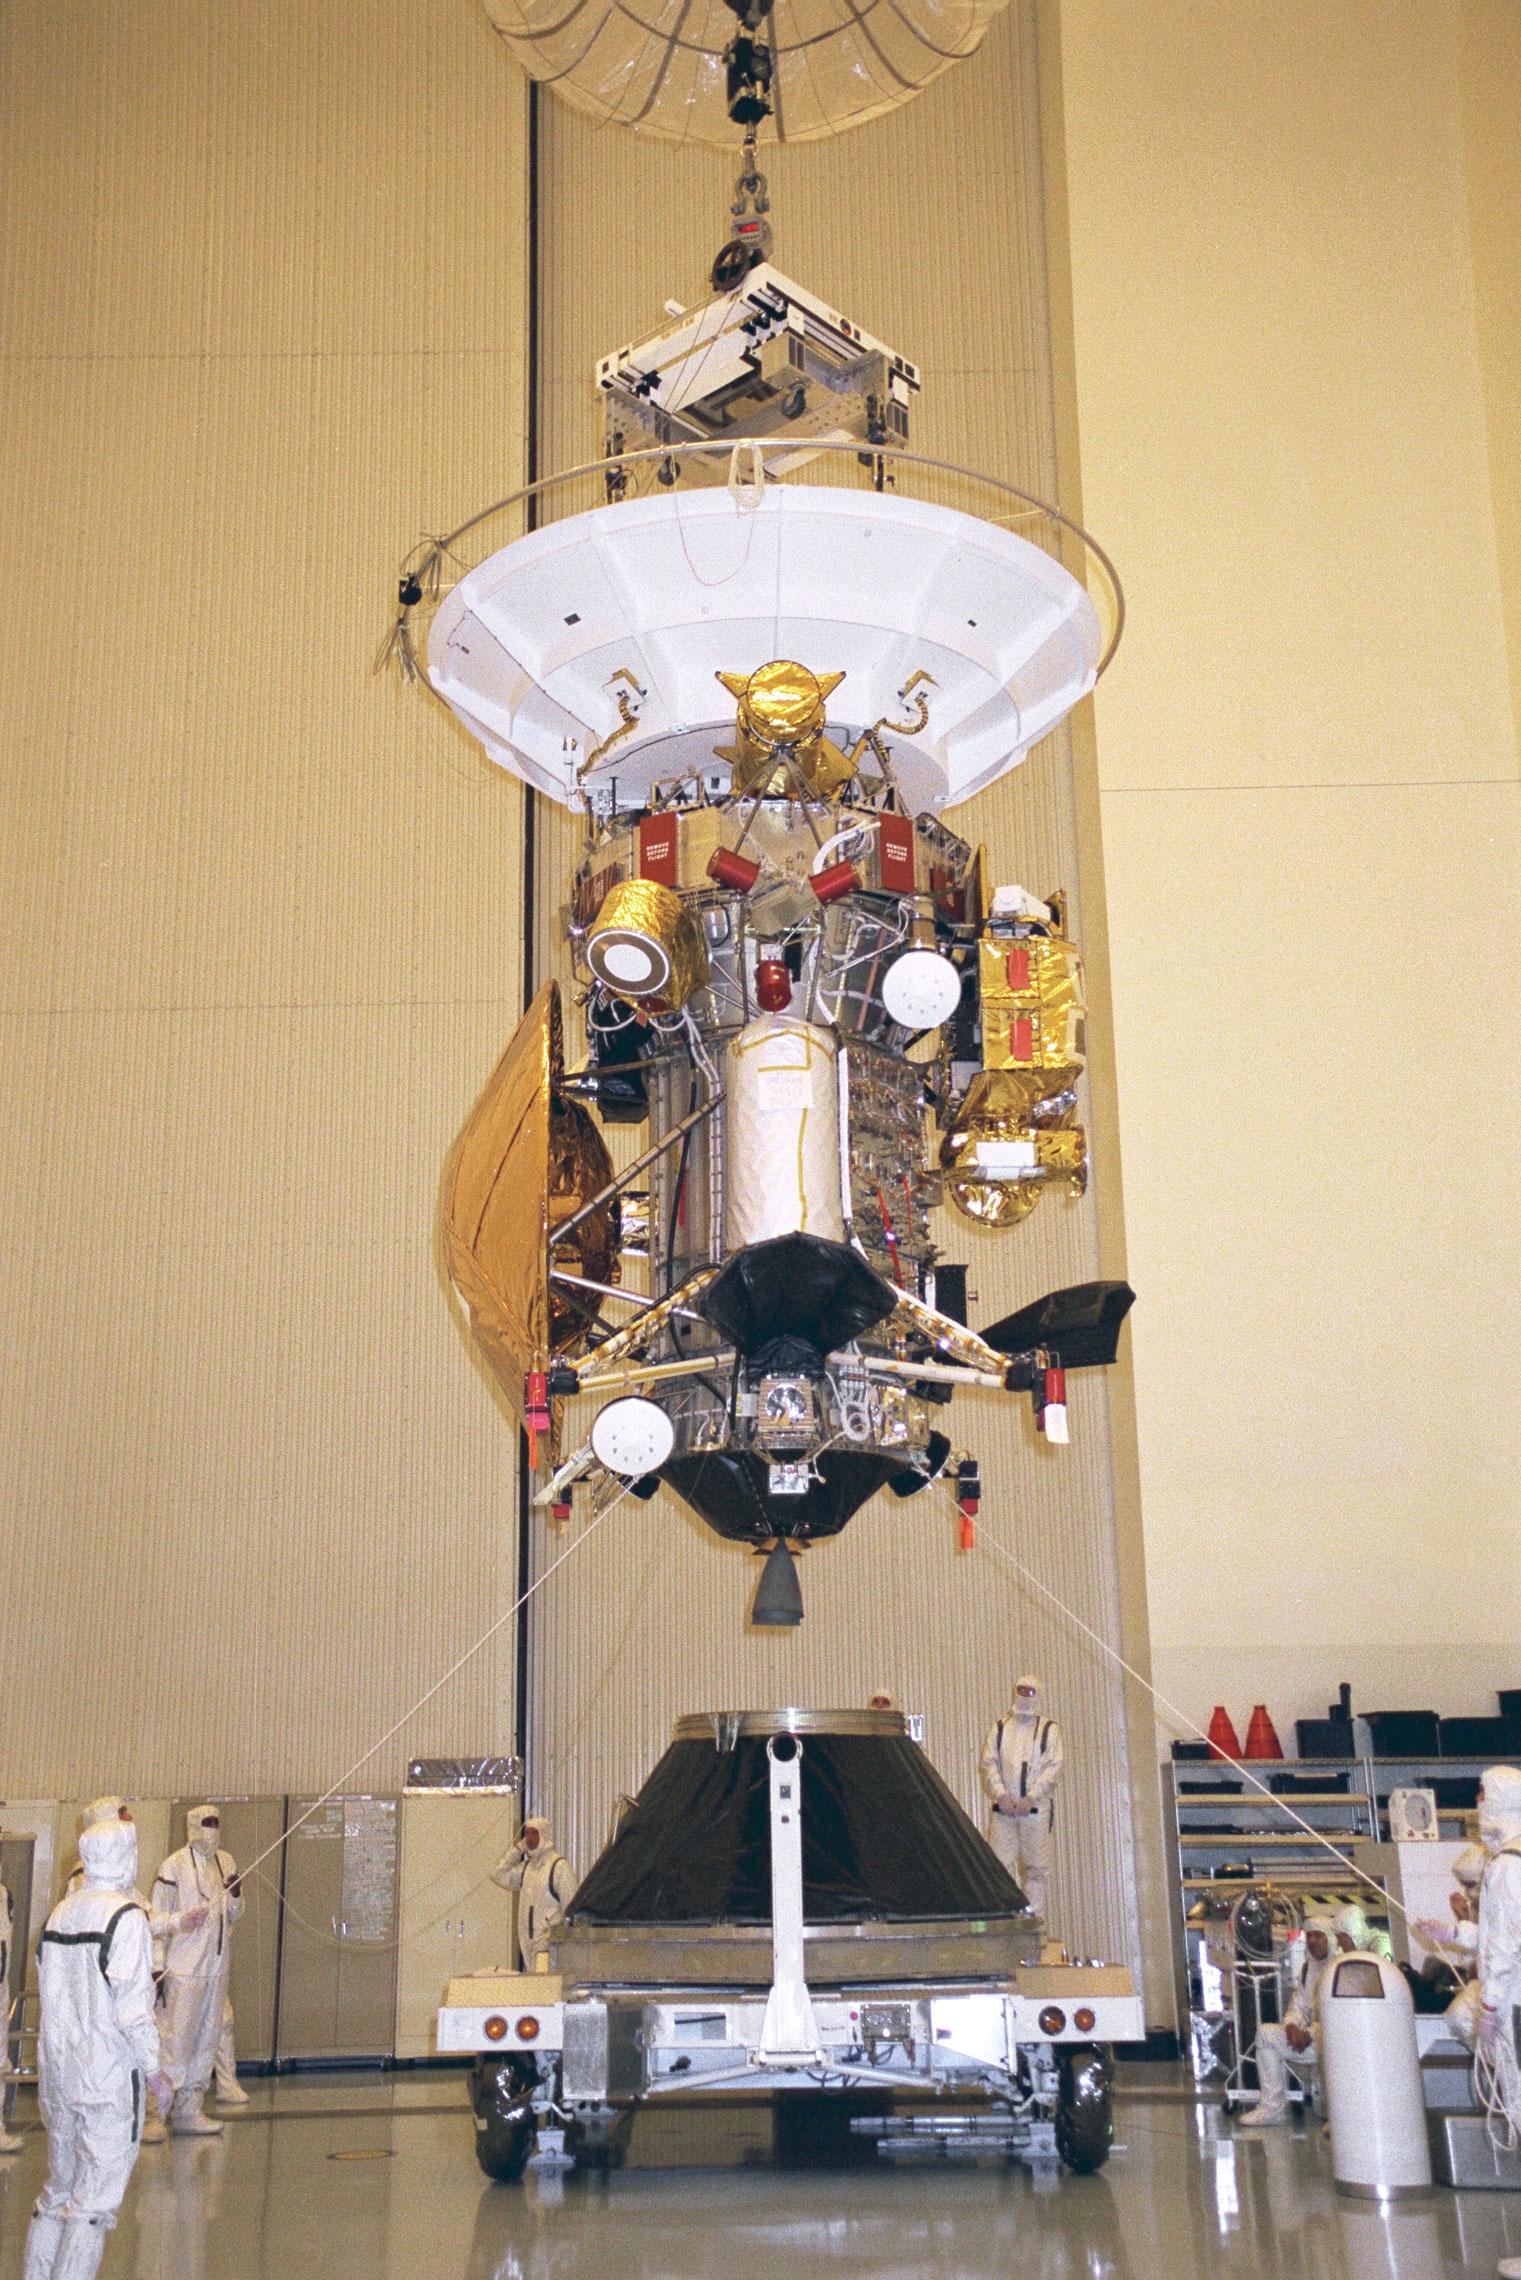
\includegraphics{cassini_being_built.jpg}}
        \end{figure}
    \end{frame}
    \begin{frame}{The Cassini Mission}
        On it's way, Cassini made several gravity assists and flew by some
        familiar objects in the sky.
    \end{frame}
    \begin{frame}{The Cassini Mission}
        \begin{figure}
            \resizebox{\textwidth}{!}{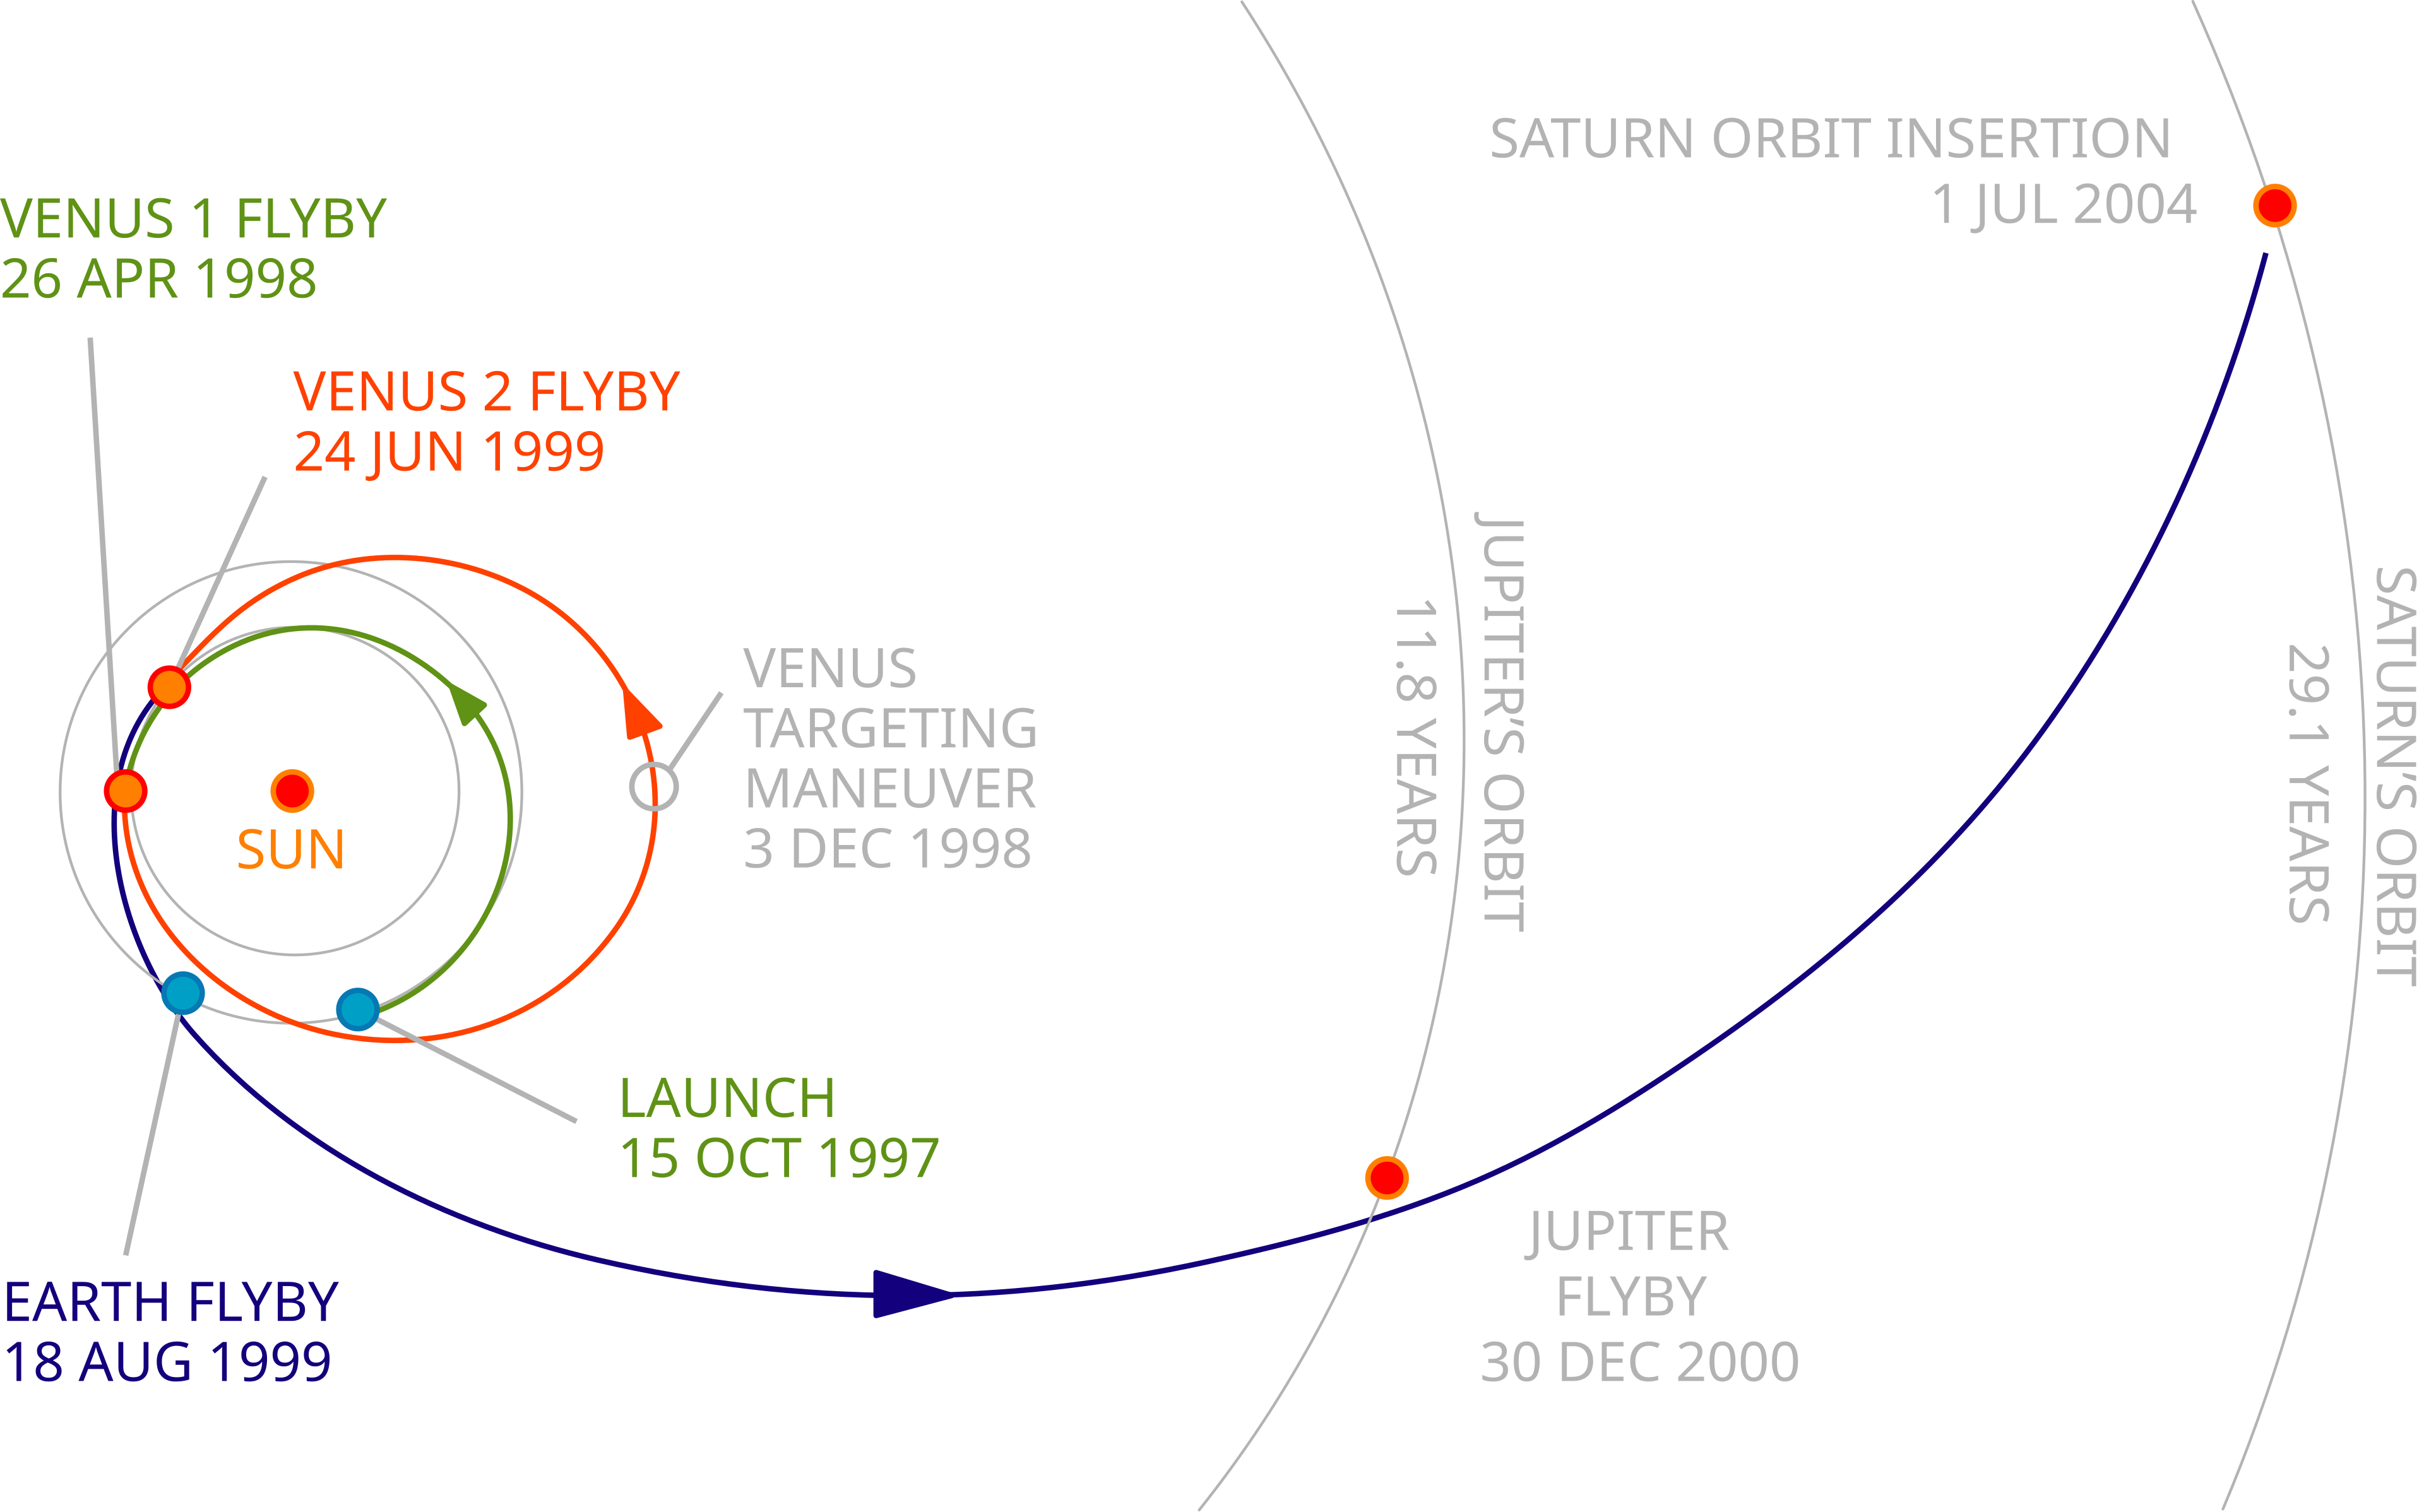
\includegraphics{cassini_trajectory.png}}
        \end{figure}
    \end{frame}
    \begin{frame}{The Cassini Mission}
        Cassini saw the moon...
        \begin{figure}
            \resizebox{!}{0.7\textheight}{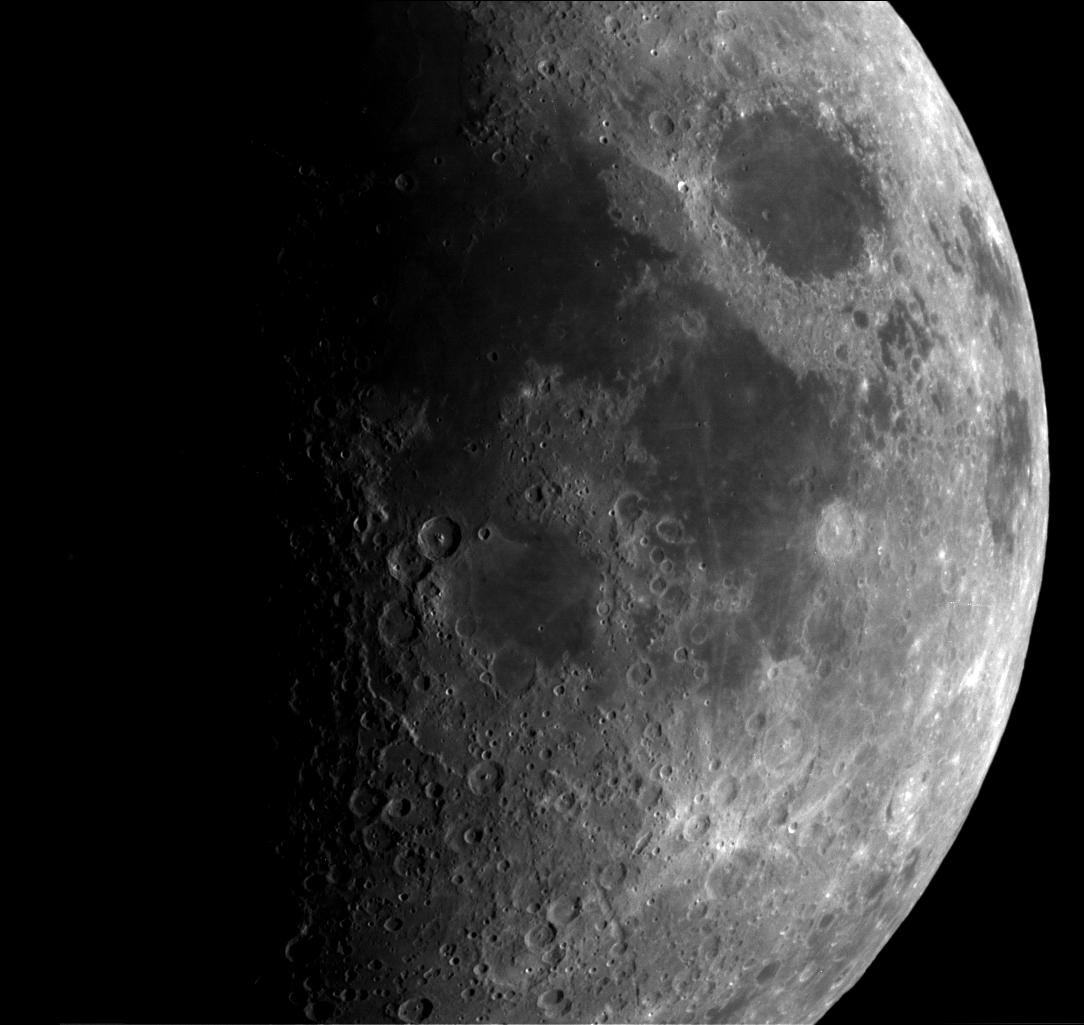
\includegraphics{moon_from_cassini.png}}
        \end{figure}
    \end{frame}
    \begin{frame}{The Cassini Mission}
        Cassini saw Jupiter...
        \begin{figure}
            \resizebox{!}{0.7\textheight}{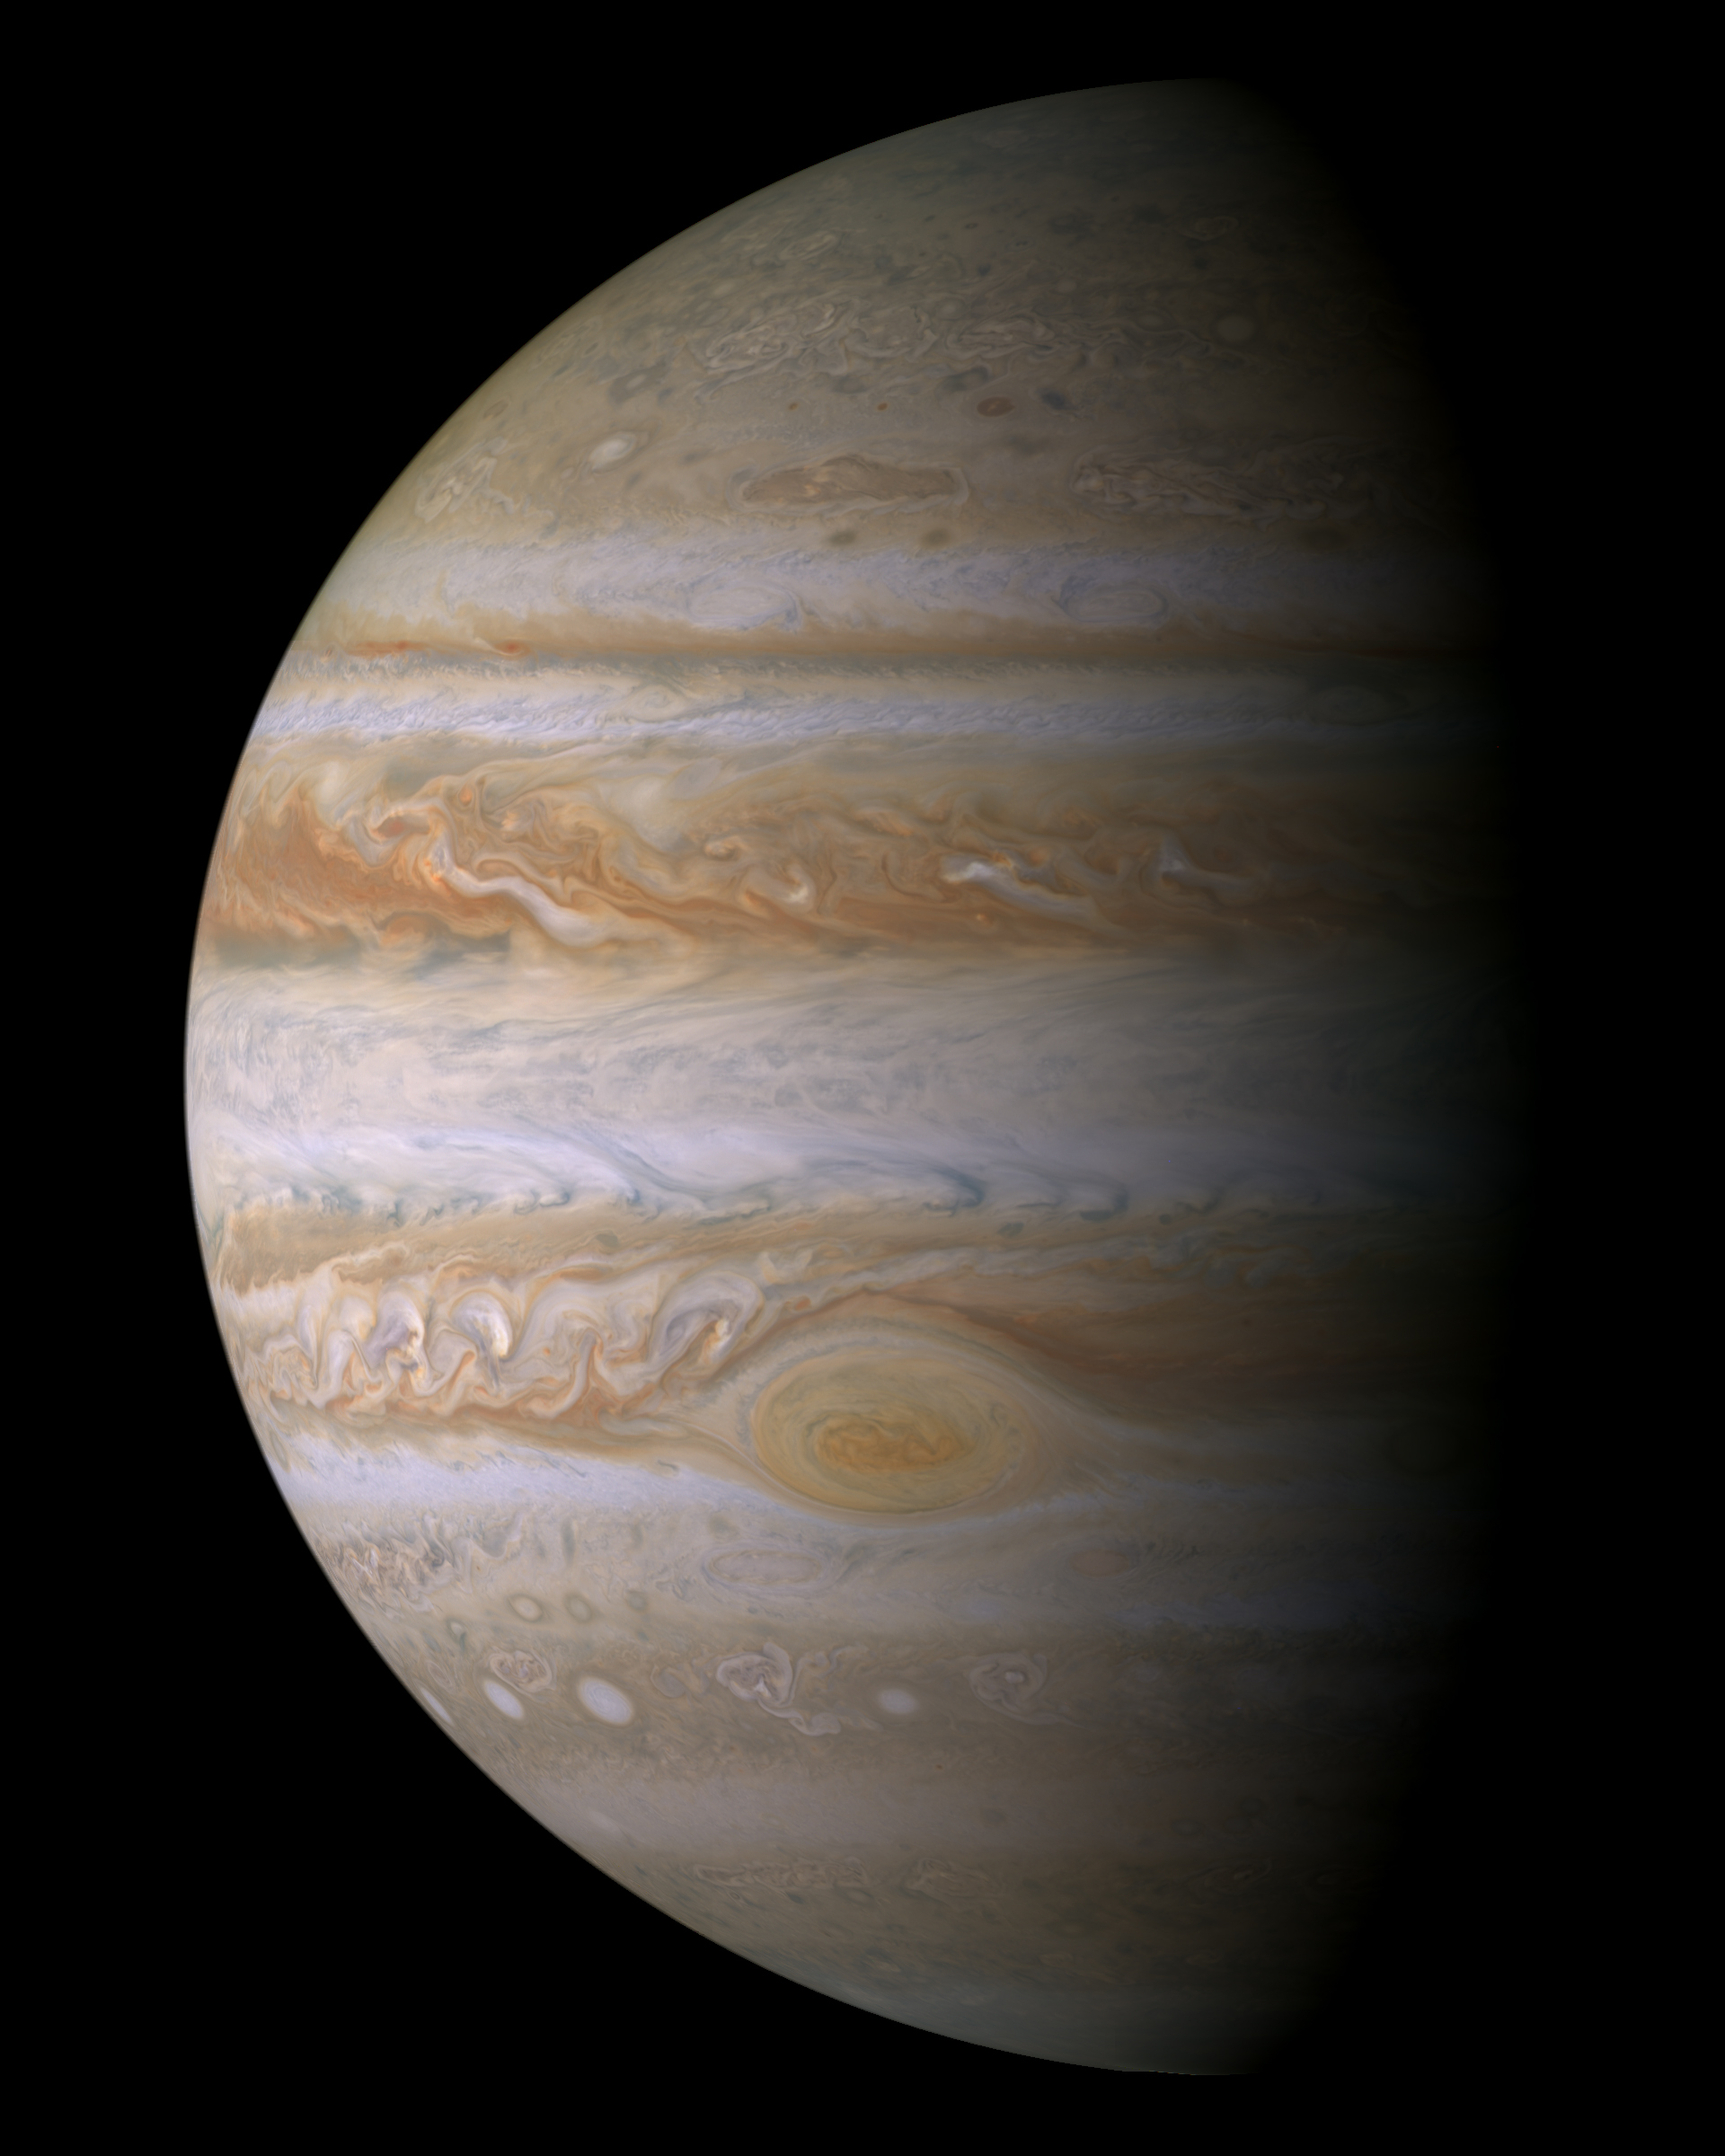
\includegraphics{jupiter_from_cassini.jpg}}
        \end{figure}
    \end{frame}
    \begin{frame}{The Cassini Mission}
        Before finally arriving at Saturn.
        \begin{figure}
            \resizebox{\textwidth}{!}{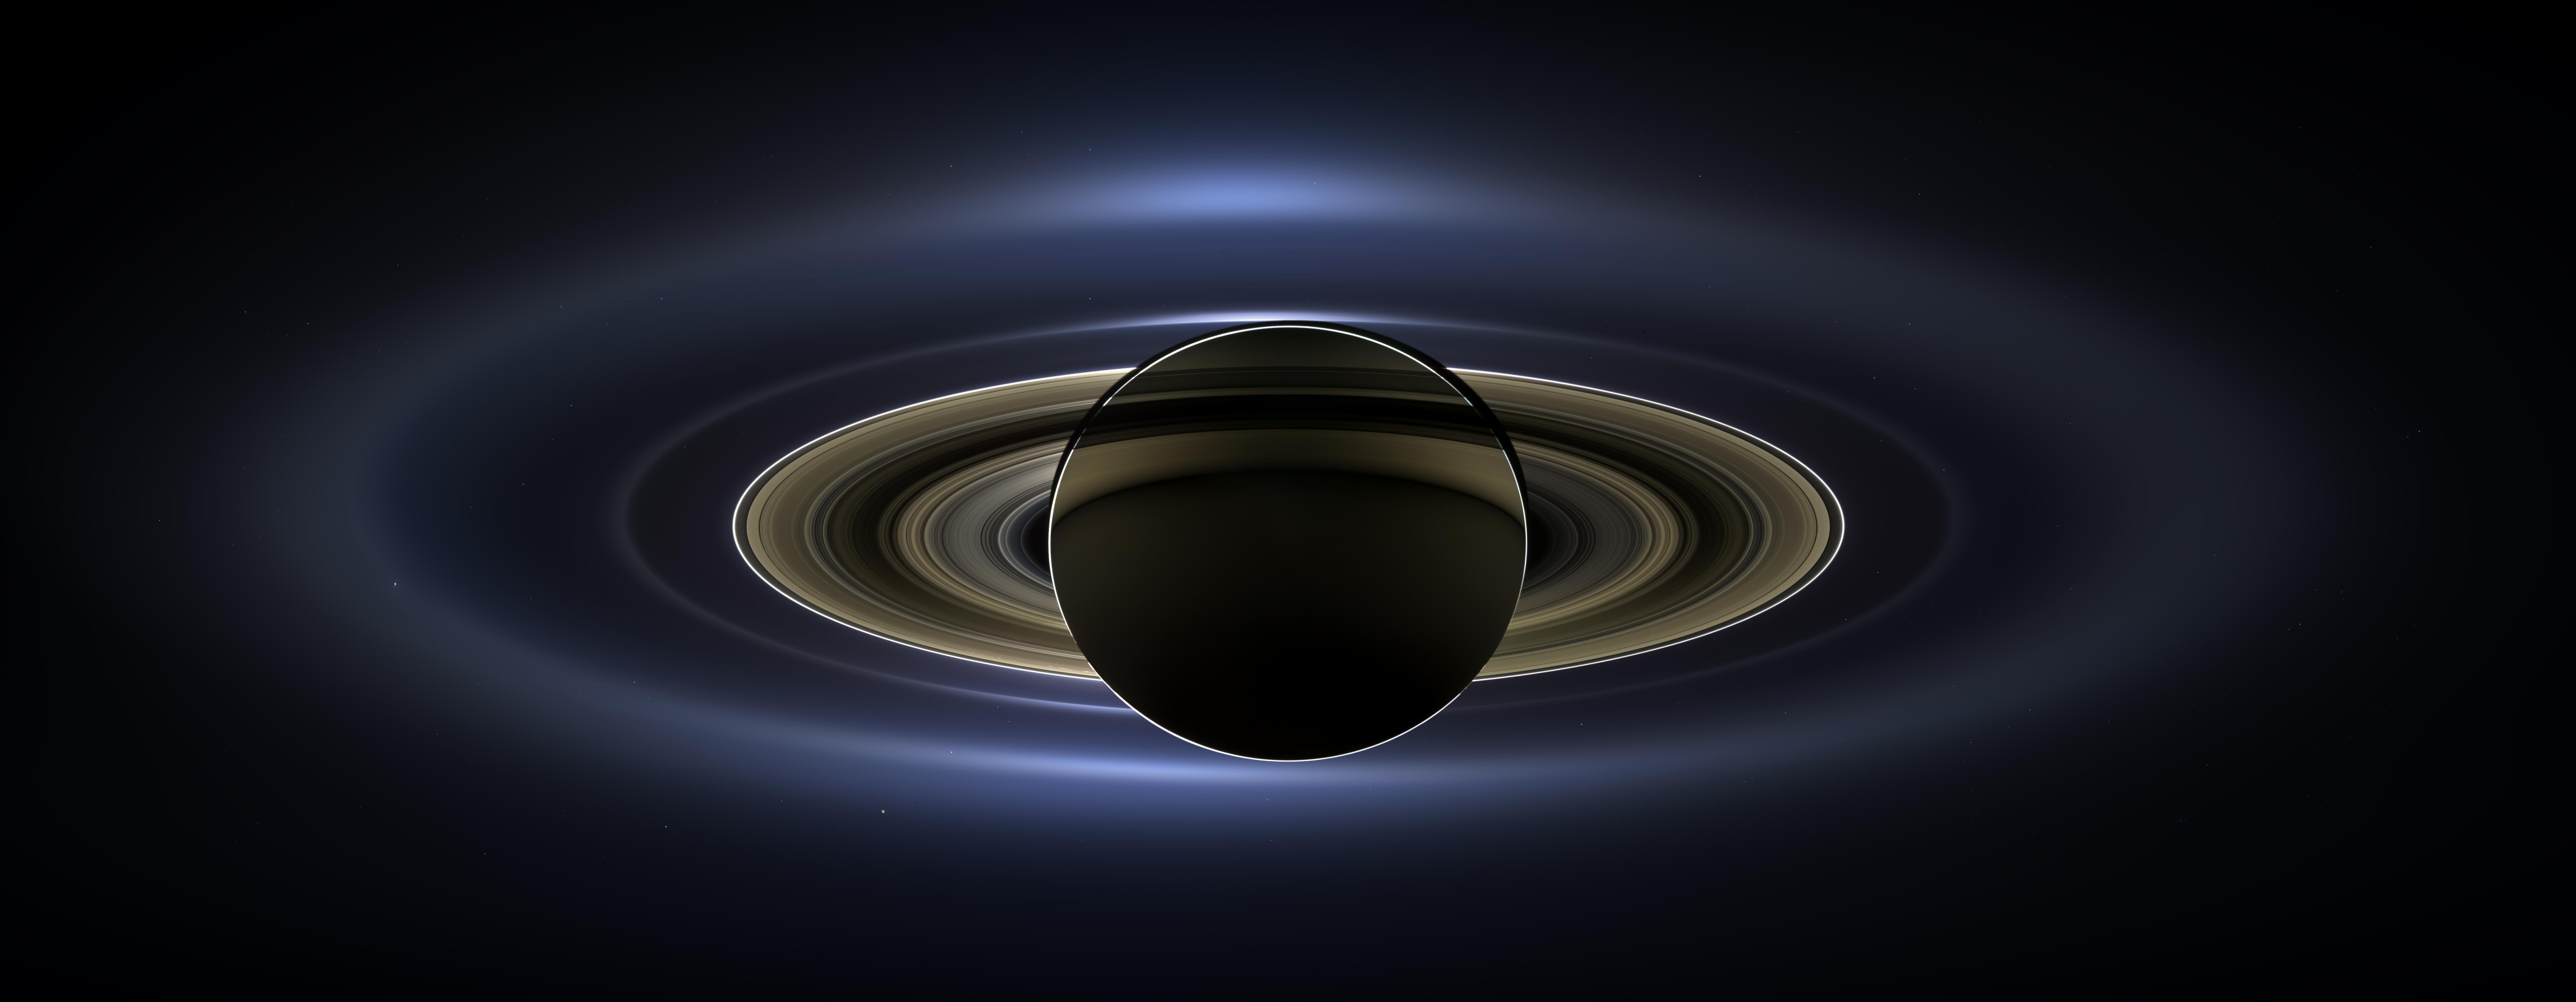
\includegraphics{sun_behind_saturn.jpg}}
        \end{figure}
    \end{frame}
    \begin{frame}{The Cassini Mission}
        And with Cassini's arrival came a plethora of new discoveries.
        \begin{figure}
            \resizebox{!}{0.8\textheight}{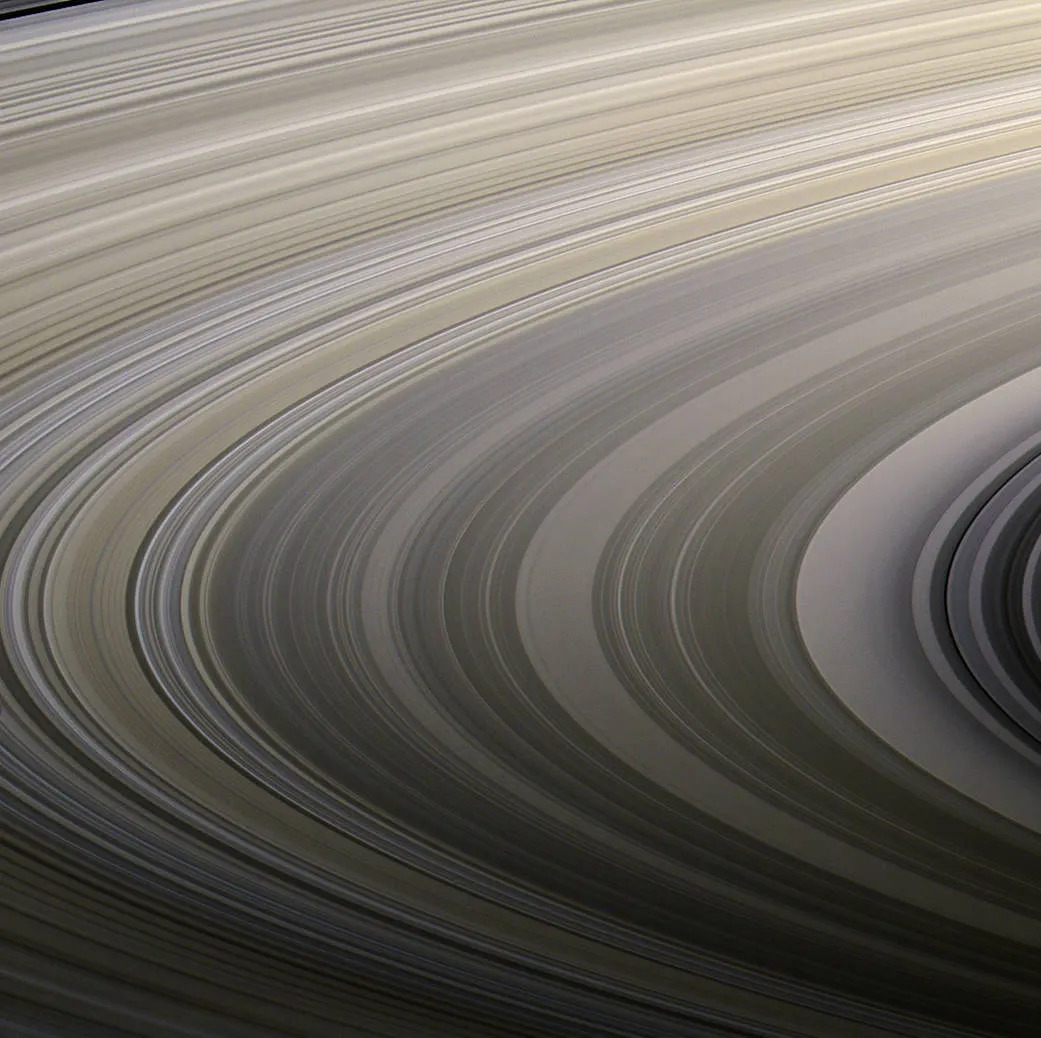
\includegraphics{rings_of_saturn.jpg}}
        \end{figure}
    \end{frame}
    \begin{frame}{The Cassini Mission}
        As Cassini orbited Saturn, occasionally its rings fell between the
        the probe and Earth. This phenomenon is called an \textit{occultation}.
        Radio waves in the Ka, X, and S bands sent from Cassini to Earth
        were then diffracted by the rings, and one observes a diffraction
        pattern on Earth. The goal is to reconstruct the ring profile from this
        diffracted pattern using Fourier optics.
    \end{frame}
    \begin{frame}{The Model}
        We can model the diffraction pattern with the good ole wave equation.
        After ``scalarizing'' (transitioning to the Helmholtz equation), we can
        obtain an integral formula for the (complex) diffraction profile:
        \begin{equation}
            \hat{T}(\rho_{0},\,\phi_{0})
            =
            \frac{\mu_{0}}{i\lambda}
            \int_{0}^{\infty}
                \int_{0}^{2\pi}
                    \rho{T}(\rho,\,\phi)\,
                    \frac{%
                        \exp\left(i\psi\right)
                    }{%
                        \|\mathbf{R}-\boldsymbol{\rho}\|
                    }\,\textrm{d}\phi\,\textrm{d}\rho
        \end{equation}
    \end{frame}
    \begin{frame}{The Model}
        Here, $\mathbf{R}$ is the position vector for Cassini,
        $\boldsymbol{\rho}=(\rho,\,\phi)$ is the dummy variable of integration,
        $\boldsymbol{\rho}_{0}=(\rho_{0},\,\phi_{0})$ is the point in the
        ring plane where the line of sight from Cassini to Earth intersects,
        $\mu_{0}$ is the \textit{ubiquity factor},
        and $\lambda$ is the wavelength.
    \end{frame}
    \begin{frame}{The Model}
        \begin{figure}
            \resizebox{\textwidth}{!}{\includegraphics{fresnel_diffraction_geometry_saturn_001}}
        \end{figure}
    \end{frame}
    \begin{frame}{The Model}
        The most important quantities in this equation
        (the Rayleigh-Sommerfeld equation) are $T$, the (normalized) complex
        transmittance, and $\psi$, the \textit{Fresnel phase}:
        \begin{equation}
            \psi
            =
            \frac{2\pi}{\lambda}
            \left(
                \|\mathbf{R}-\boldsymbol{\rho}\|
                -
                \mathbf{u}\cdot\left(
                    \mathbf{R}-\boldsymbol{\rho}
                \right)
            \right)
        \end{equation}
        where $\mathbf{u}$ is the unit vector from $\mathbf{R}$ to
        $\boldsymbol{\rho}_{0}$:
        \begin{equation}
            \mathbf{u}
            =
            \frac{%
                \mathbf{R}-\boldsymbol{\rho}_{0}%
            }{%
                \|\mathbf{R}-\boldsymbol{\rho}_{0}\|%
            }
        \end{equation}
    \end{frame}
    \begin{frame}{The Model}
        As is, there's not much that can be done without introducing more
        assumptions. The rings of Saturn are very symmetric, so we assume
        $T(\rho,\,\phi)=T(\rho)$. The double integral simplifies to:
        \begin{equation}
            \hat{T}(\rho_{0})
            =
            \frac{\mu_{0}}{i\lambda}
            \int_{0}^{\infty}
                \rho{T}(\rho)
                \int_{0}^{2\pi}
                    \frac{%
                        \exp\left(i\psi\right)
                    }{%
                        \|\mathbf{R}-\boldsymbol{\rho}\|
                    }\,\textrm{d}\phi\,\textrm{d}\rho
        \end{equation}
    \end{frame}
    \begin{frame}{The Model}
        This inner integral is of the form:
        \begin{equation}
            I
            =
            \int_{a}^{b}
                e^{if(t)}\textrm{d}t
        \end{equation}
        Since $f$ grows faster-than-linear, most of the contribution comes
        from where $f$ is roughly stationary. That is, as $f$ grows
        faster and faster, $e^{if(t)}$ starts to oscillate rapidy, meaning
        the regions under the curve start to cancel each other and
        contribute little to the integral.
    \end{frame}
    \begin{frame}{The Model}
        By applying this to the Fresnel transform, we get:
        \begin{equation}
            \hat{T}(\rho_{0})
            =
            \frac{1-i}{\sqrt{2}}\frac{\mu_{0}}{i\lambda}
            \int_{0}^{\infty}
                \rho
                T(\rho)
                \sqrt{\frac{2\pi}{|\psi^{\prime\prime}_{s}|}}
                \frac{\exp(i\psi_{s})}{\|\mathbf{R}-\boldsymbol{\rho}_{s}\|}\,
                \textrm{d}\rho
        \end{equation}
        where the subscript $s$ denotes the evaluation of the term at
        $\phi=\phi_{s}$, the solution to $\partial\psi/\partial\phi=0$.
    \end{frame}
    \begin{frame}{The Model}
        Some more simplifications can get us to:
        \begin{equation}
            \hat{T}(\rho_{0})
            \approx
            \frac{1-i}{2F}
            \int_{0}^{\infty}
                T(\rho)\exp(i\psi_{s})\,\textrm{d}\rho
        \end{equation}
        where $F$ is the so-called \textit{Fresnel scale}.
    \end{frame}
    \begin{frame}{The Fresnel Approximation}
        If the angle between the ring plane and the line of sight to Earth is
        large, a decent approximation to $\psi_{s}$ can be found by applying
        a single iteration of Newton's method to the guess $\phi_{s}=\phi_{0}$,
        and then using the Quadratic Taylor polynomial for this expression
        expanded about $\rho_{0}$. This is the classic Fresnel approximation:
        \begin{equation}
            \hat{T}(\rho_{0})
            \approx
            \frac{1+i}{2F}
            \int_{0}^{\infty}
                T(\rho)
                \exp\left(
                    \frac{i\pi}{2}\big(\frac{\rho-\rho_{0}}{F}\big)^{2}
                \right)\,\textrm{d}\rho
        \end{equation}
    \end{frame}
    \begin{frame}{The Fresnel Approximation}
        This integral is in the form of a convolution. Using Fourier transforms,
        we can get an inverse formula as follows:
        \begin{equation}
            T(\rho)
            \approx
            \frac{1-i}{2F}
            \int_{0}^{\infty}
                \hat{T}(\rho_{0})
                \exp\left(
                    -\frac{i\pi}{2}\big(\frac{\rho-\rho_{0}}{F}\big)^{2}
                \right)\,\textrm{d}\rho_{0}
        \end{equation}
        This works provided the opening angle, $B$, is large.
        Uranus is tilted almost completely on its side (about $89^{\circ}$),
        meaning the Voyager flyby of Uranus provides the best example of where
        this method applies.
    \end{frame}
    \begin{frame}{The Fresnel Approximation}
        \begin{figure}
            \resizebox{\textwidth}{!}{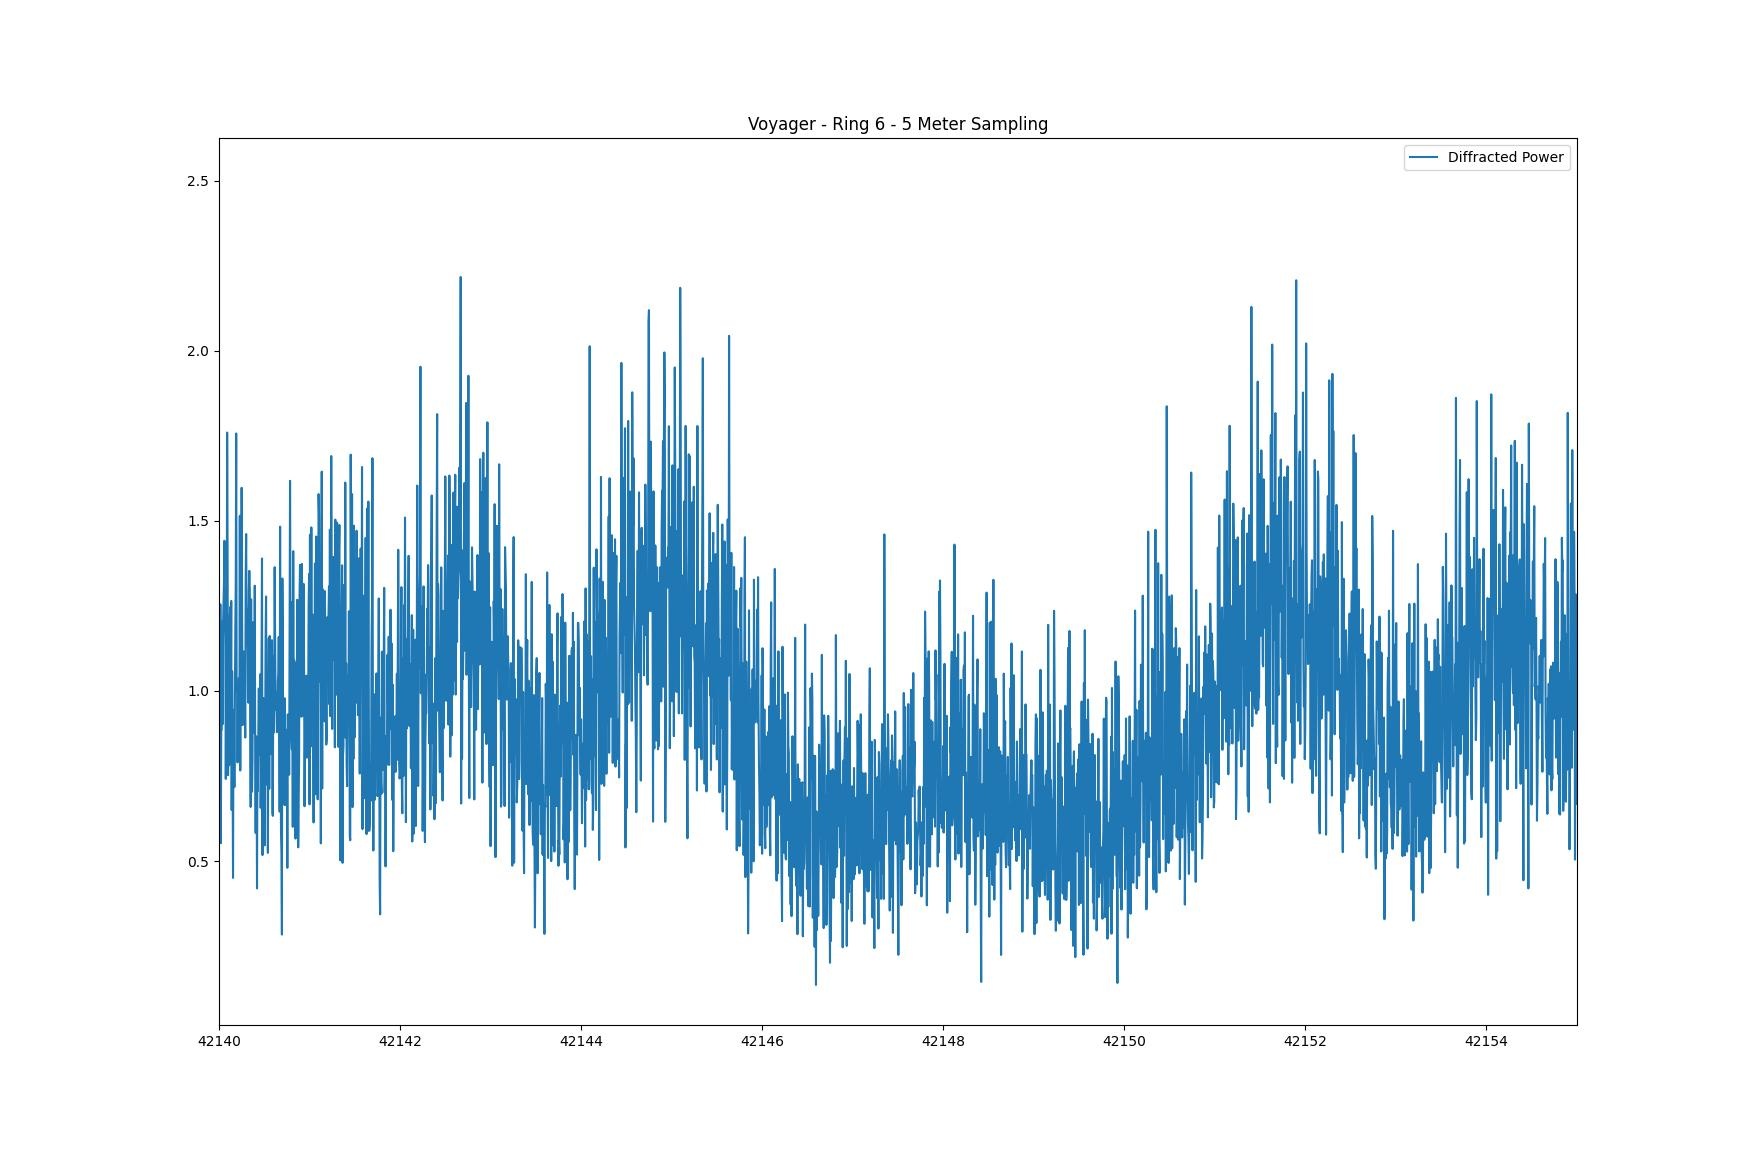
\includegraphics{voyager_ring_6_diffracted_power.png}}
        \end{figure}
    \end{frame}
    \begin{frame}{The Fresnel Approximation}
        \begin{figure}
            \resizebox{\textwidth}{!}{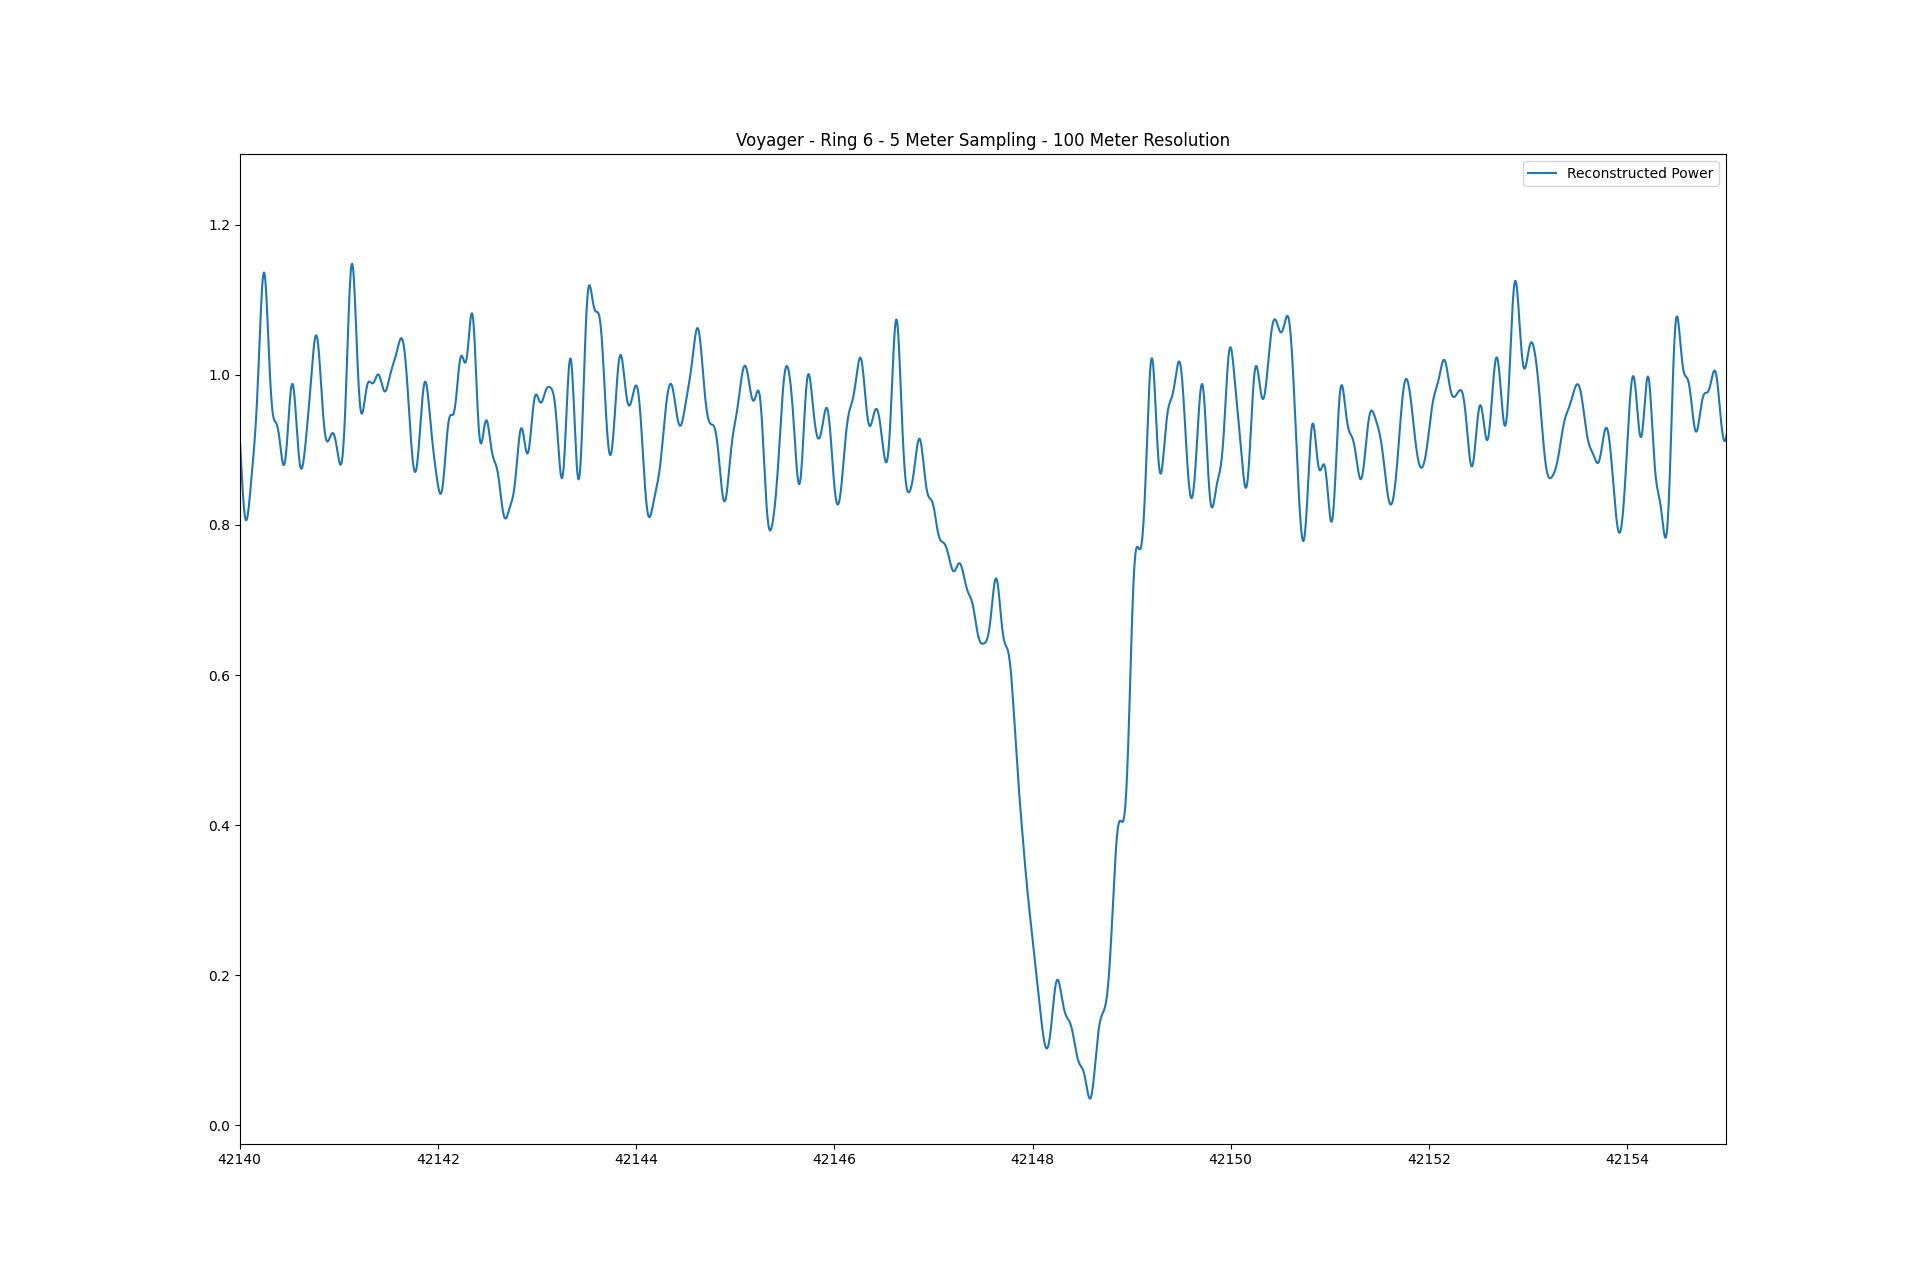
\includegraphics{voyager_ring_6_reconstructed_power_100m.png}}
        \end{figure}
    \end{frame}
    \begin{frame}{The Fresnel Approximation}
        \begin{figure}
            \resizebox{\textwidth}{!}{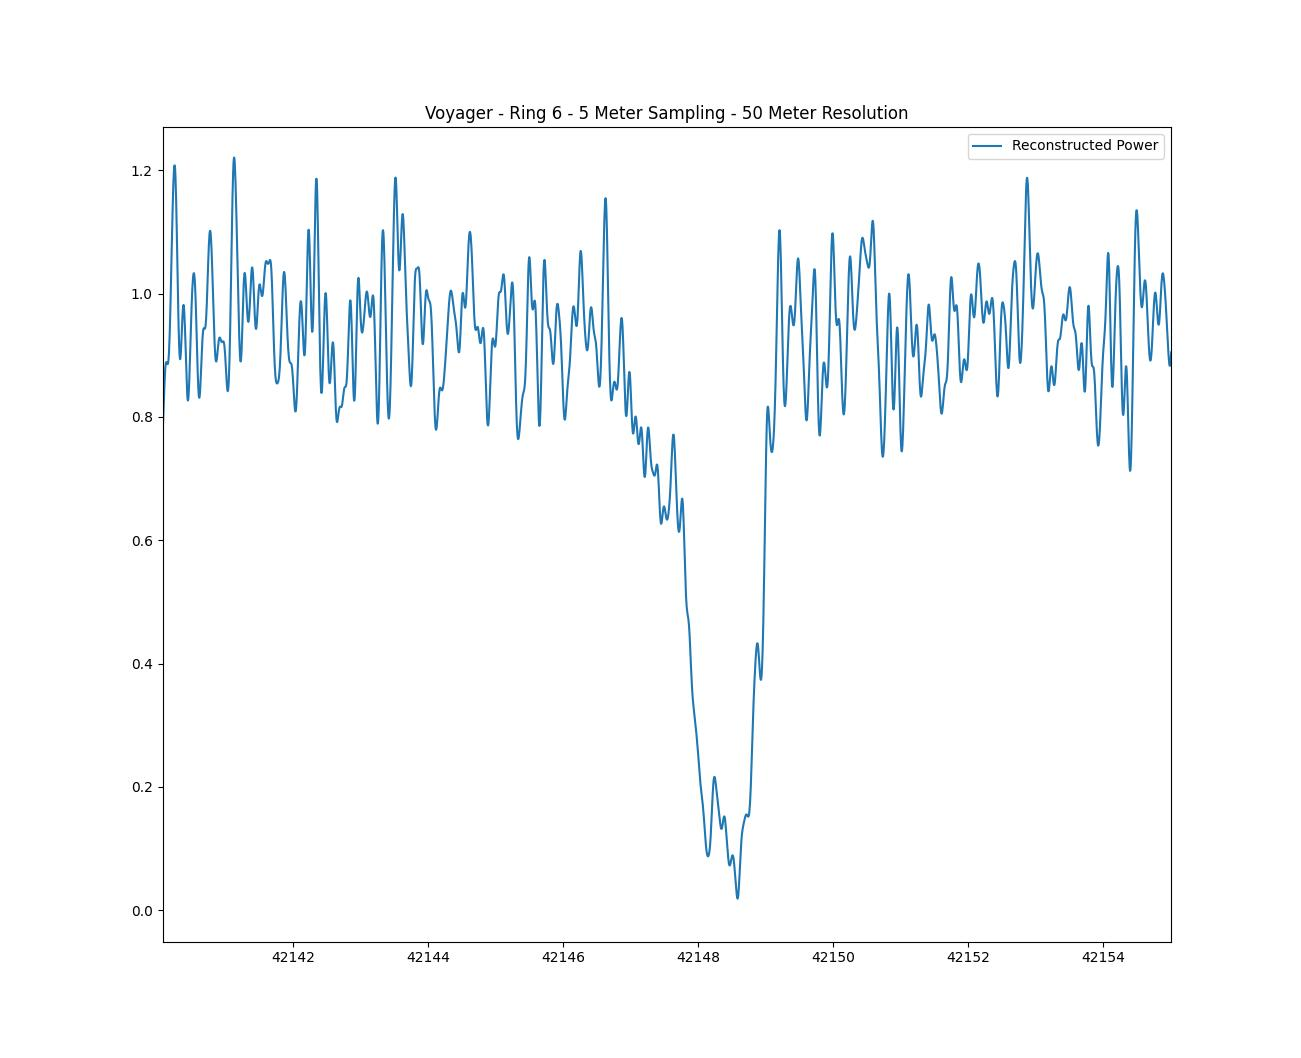
\includegraphics{voyager_ring_6_reconstructed_power_50m.png}}
        \end{figure}
    \end{frame}
    \begin{frame}{The Fresnel Approximation}
        When Cassini first arrived in 2004, the rings of Saturn were close to
        their maximum opening angle (about $27^{\circ}$). As it turns out,
        this angle is also small enough.
    \end{frame}
    \begin{frame}{The Fresnel Approximation}
        \begin{figure}
            \resizebox{\textwidth}{!}{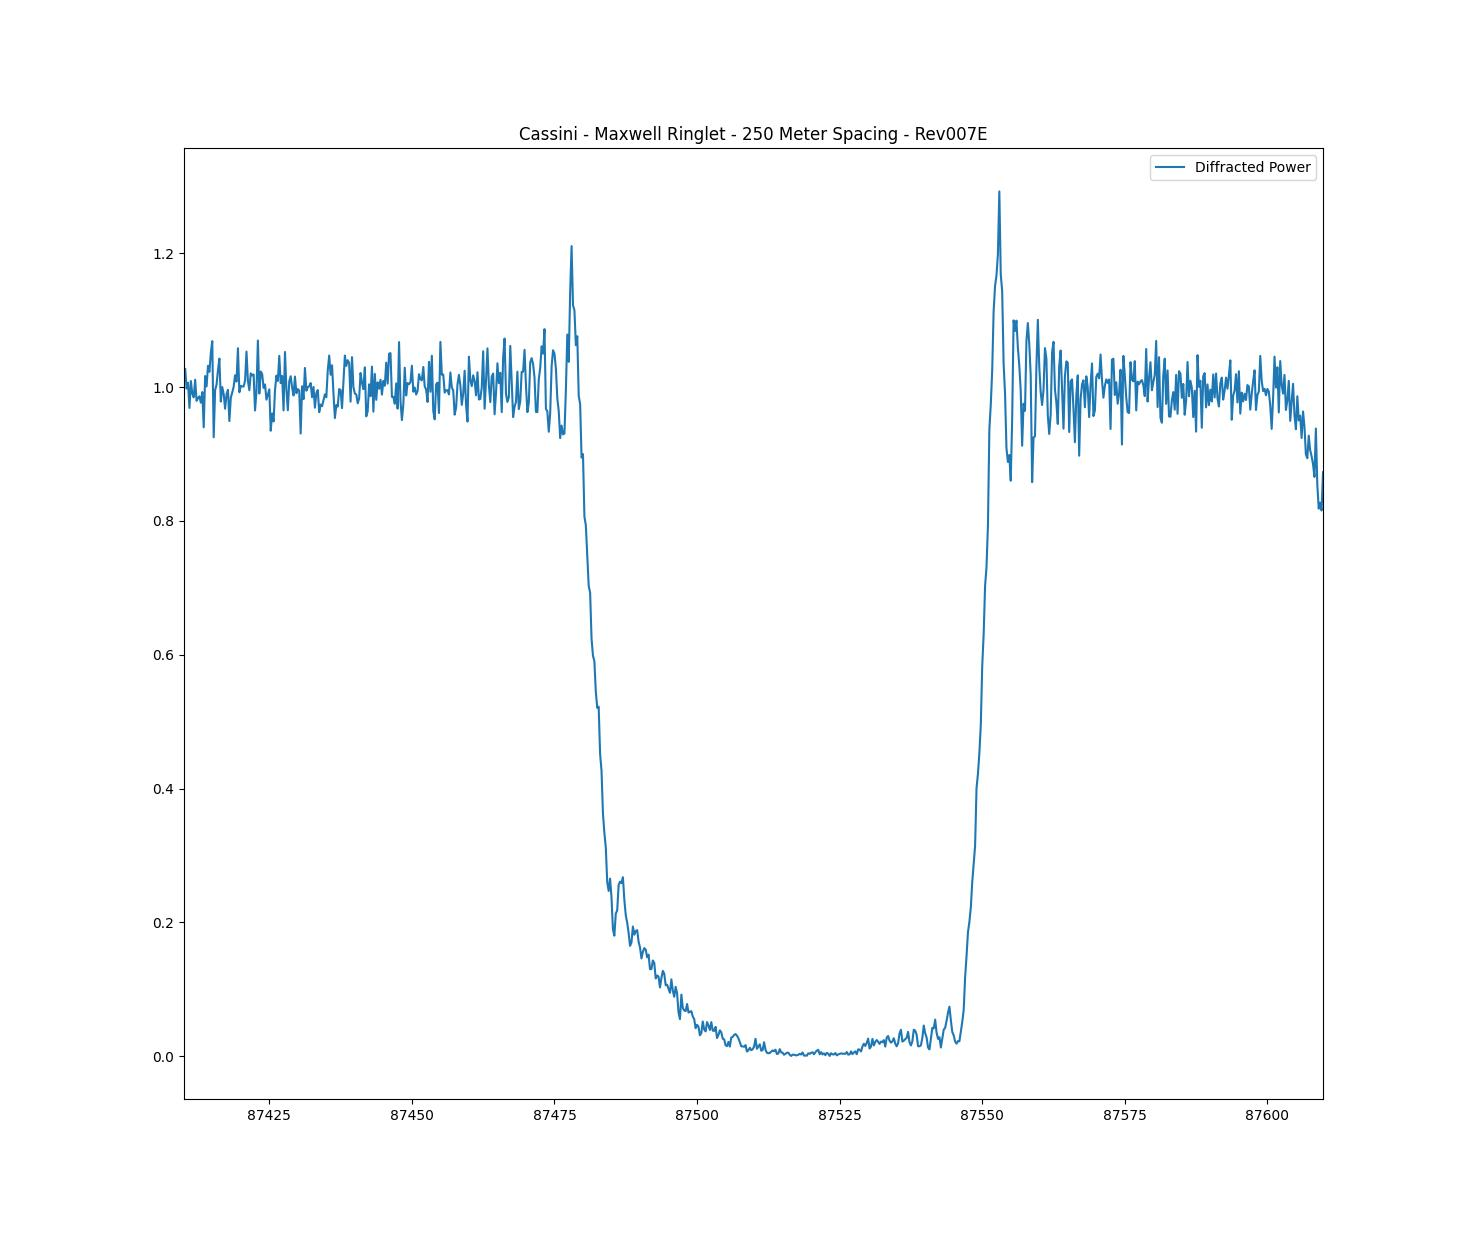
\includegraphics{cassini_maxwell_rev007e_diffracted_power_250m.png}}
        \end{figure}
    \end{frame}
    \begin{frame}{The Fresnel Approximation}
        \begin{figure}
            \resizebox{\textwidth}{!}{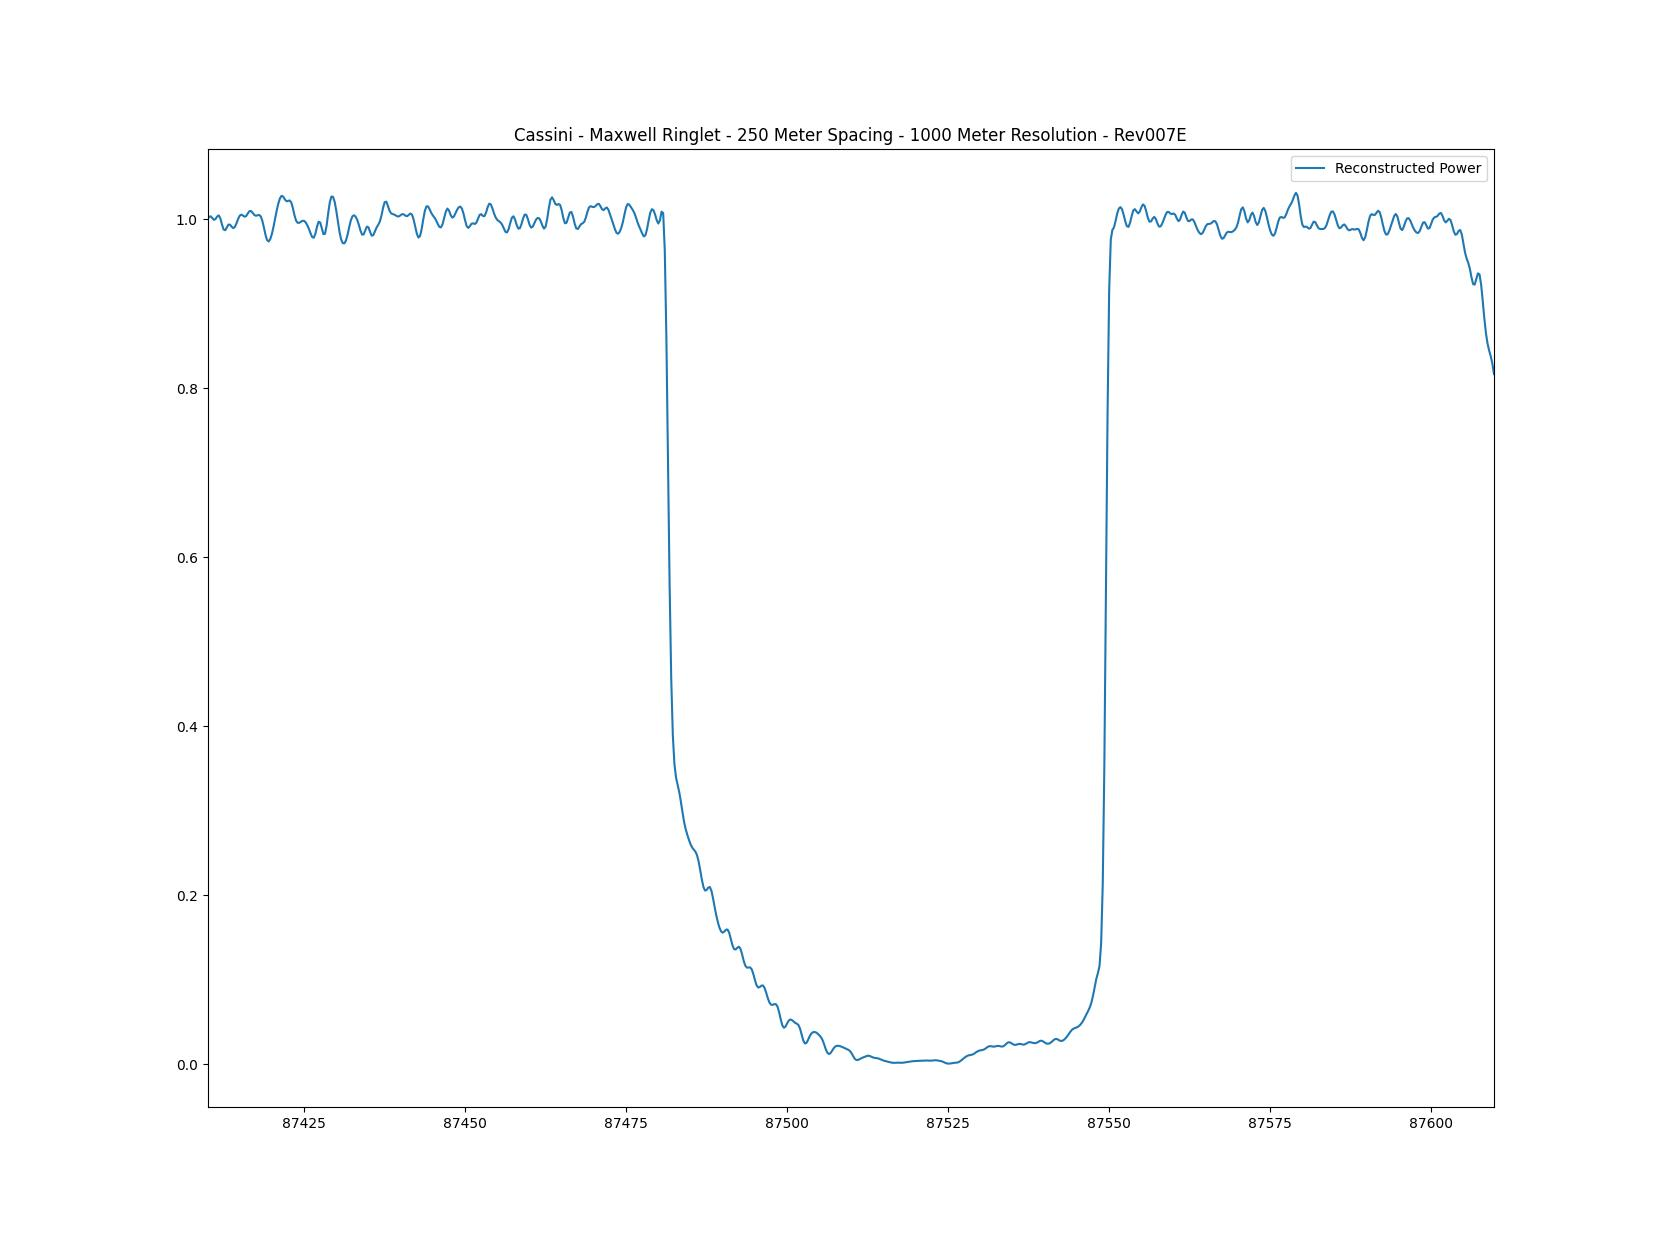
\includegraphics{cassini_maxwell_rev007e_reconstructed_power_1000m.png}}
        \end{figure}
    \end{frame}
    \begin{frame}{The Fresnel Approximation}
        Cassini did much higher sampling, but for higher resolutions we need a
        better approximation for $\psi_{s}$. Using this idea of expanding
        after applying a single iteration of Newton's method, we can obtain a
        nice formula in terms of Legendre polynomials. Higher resolutions can
        be obtained quite easily.
    \end{frame}
    \begin{frame}{The Fresnel Approximation}
        \begin{figure}
            \resizebox{\textwidth}{!}{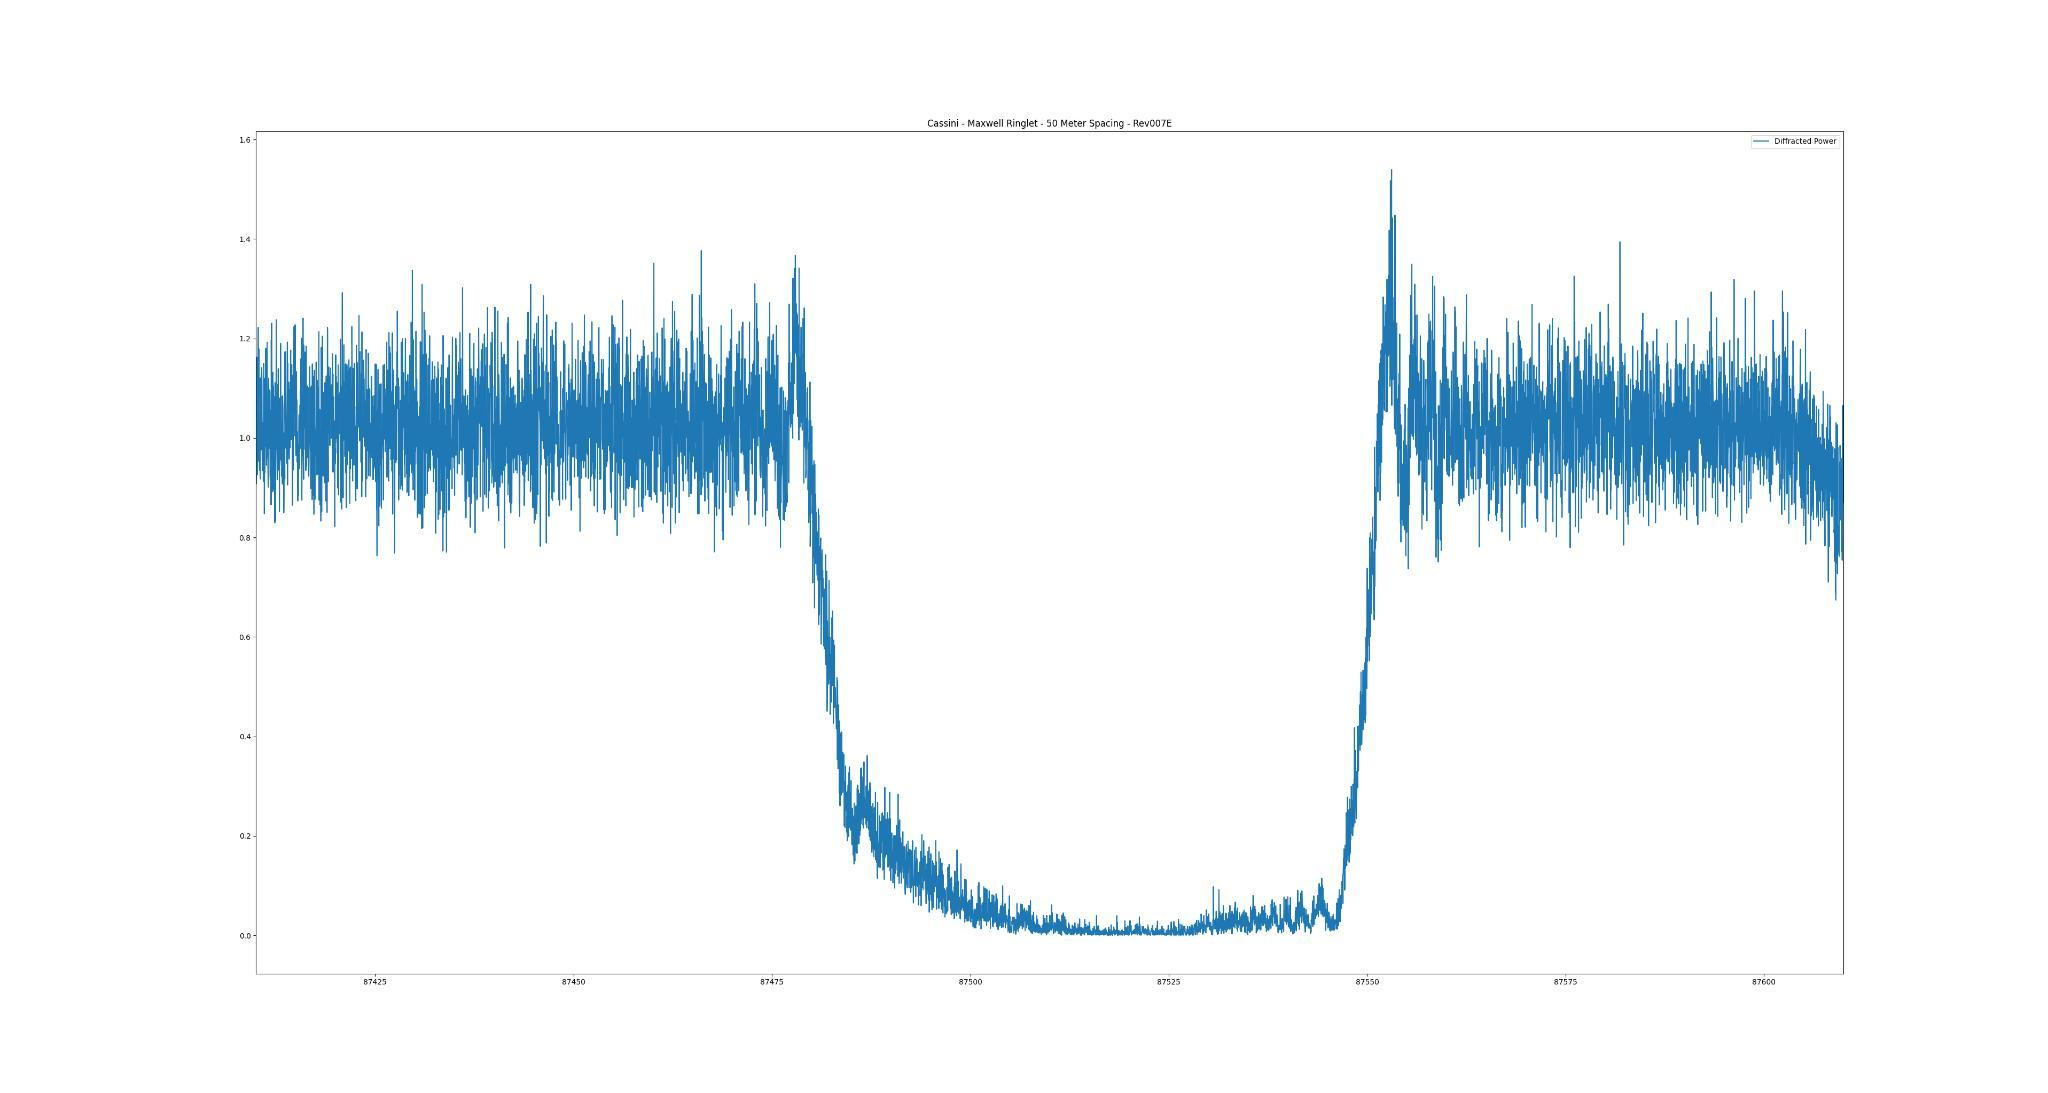
\includegraphics{cassini_maxwell_rev007e_diffracted_power_50m.png}}
        \end{figure}
    \end{frame}
    \begin{frame}{The Fresnel Approximation}
        \begin{figure}
            \resizebox{\textwidth}{!}{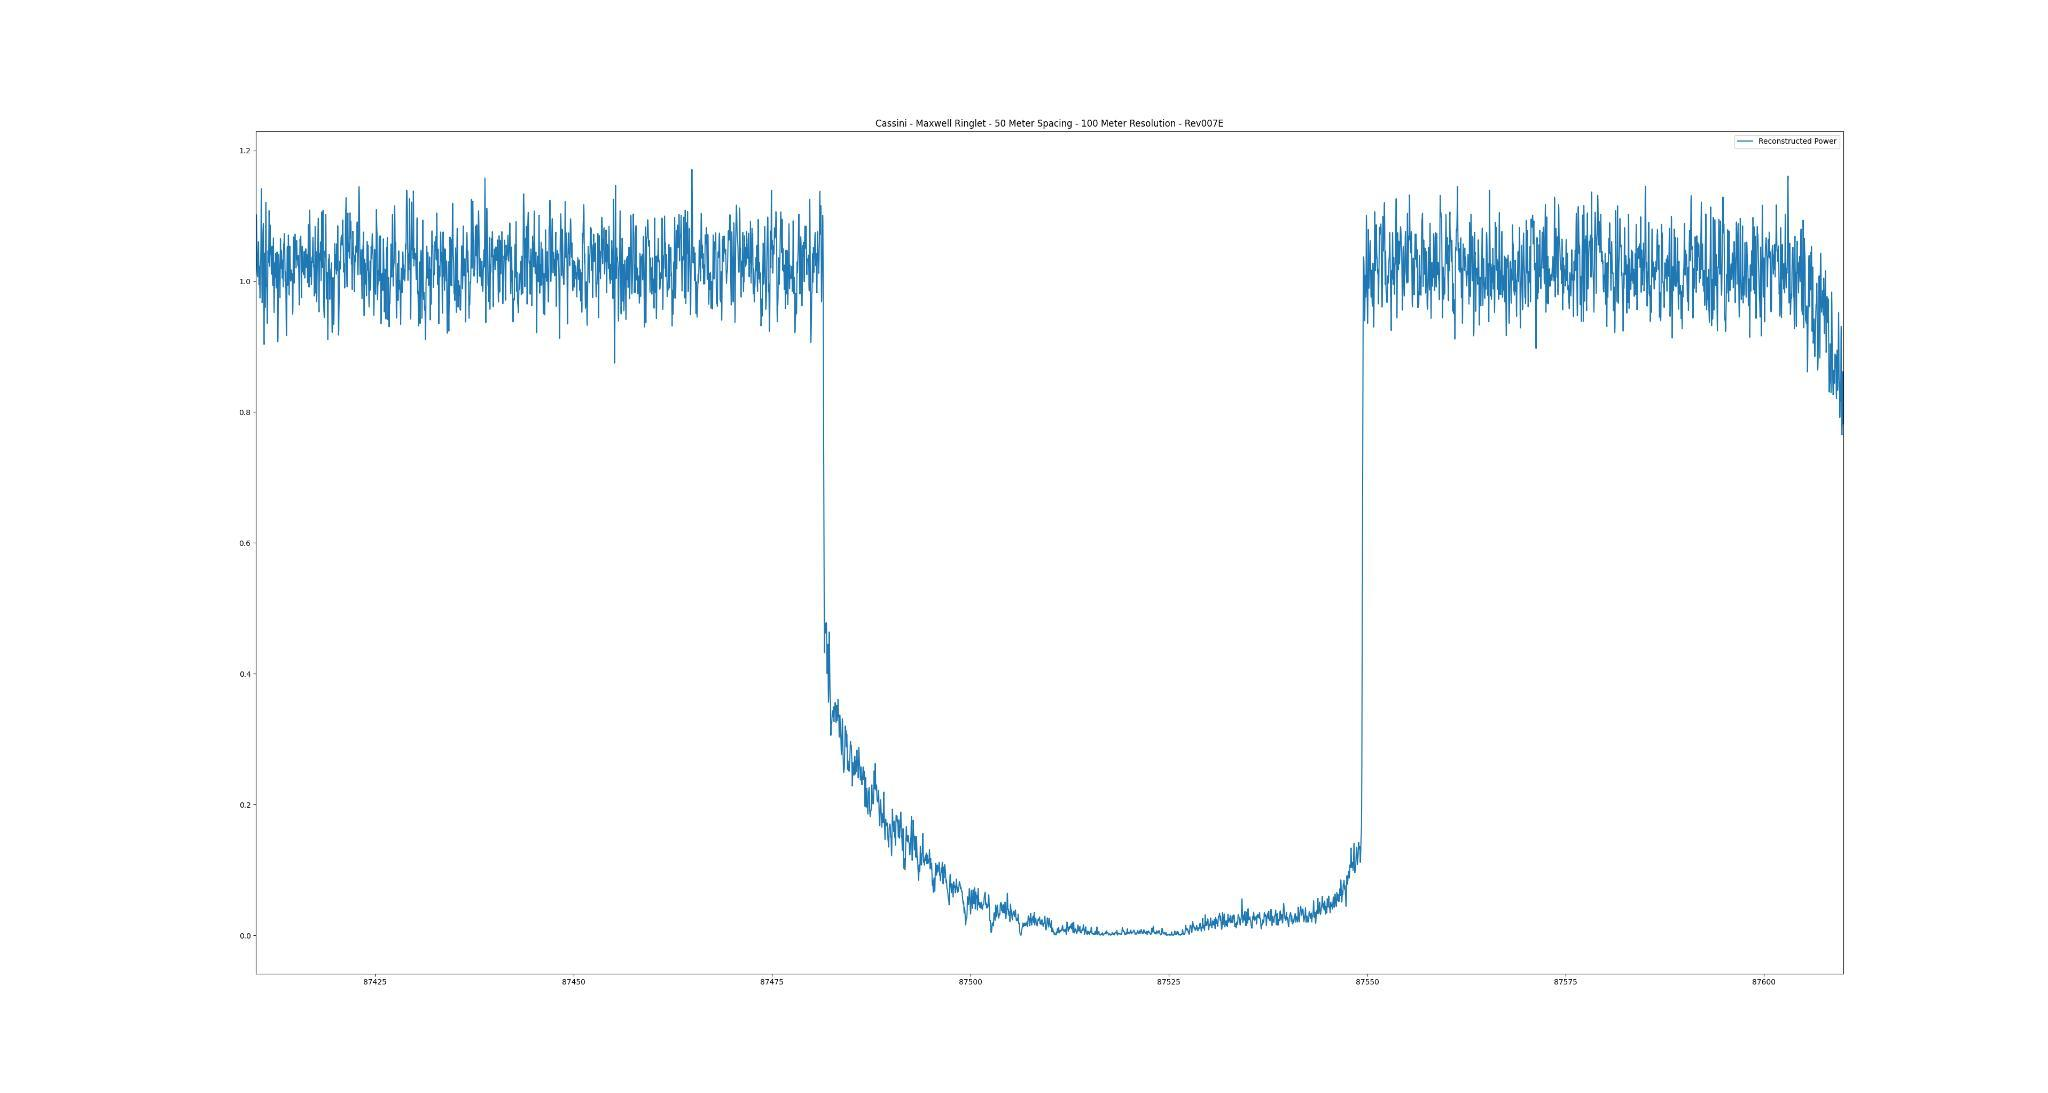
\includegraphics{cassini_maxwell_rev007e_reconstructed_power_100m.png}}
        \end{figure}
    \end{frame}
    \begin{frame}{High Resolution with Low Opening Angle}
        Several issues arise when the opening angle decreases. One of the
        data sets has $B\approx{1}^{\circ}$.
        Here are some of the problems we've encountered.
        \begin{enumerate}
            \item
                The approximation
                \begin{equation}
                    \hat{T}(\rho_{0})
                    \approx
                    \frac{1-i}{2F}
                    \int_{0}^{\infty}
                        T(\rho)\exp(i\psi_{s})\,\textrm{d}\rho
                \end{equation}
                stops working.
            \item
                Need several more iterations of Newton's method to find
                $\psi_{s}$.
            \item
                As the resolution increases, so does the window of integration,
                and eventually you include points with
                $\partial^{2}\psi/\partial\phi^{2}=0$, Newton's method diverges.
            \item
                $\psi$ grows rapidly as the window width increases.
                Numerically integrating $\exp(i\psi)$ starts to introduce
                aliasing if you're not careful.
            \item
                Summing together millions of points introduces floating-point
                round-off on the order of the number of points being summed.
        \end{enumerate}
    \end{frame}
    \begin{frame}{High Resolution with Low Opening Angle}
        Our fixes:
        \begin{enumerate}
            \item
                Use the original formula, our approximate inverse is obtained
                by swapping the variables of integration and taking the
                complex conjugate of the integrand. Hey, it works
                (evidence in a few slides)! This means we cannot use FFTs,
                since the integral equation is not a true convolution. This
                produces a 1000x slow down (ouch).
            \item
                Do between 6 and 10 iterations of Newton's method. Things are
                getting pretty slow now...
            \item
                Swap Newton's method with Halley's method
                (this actually helps performance, Halley needs fewer iterations).
            \item
                Use a (new) modified Filon quadrature for $\psi$ by numerically
                integrating via Fresnel functions.
            \item
                Replace a normal sum with a Kahan sum. This puts the error
                back to roughly double precision.
        \end{enumerate}
    \end{frame}
    \begin{frame}{High Resolution with Low Opening Angle}
        Let's use this and look at a \textit{boring} part of the rings.
        \begin{figure}
            \resizebox{\textwidth}{!}{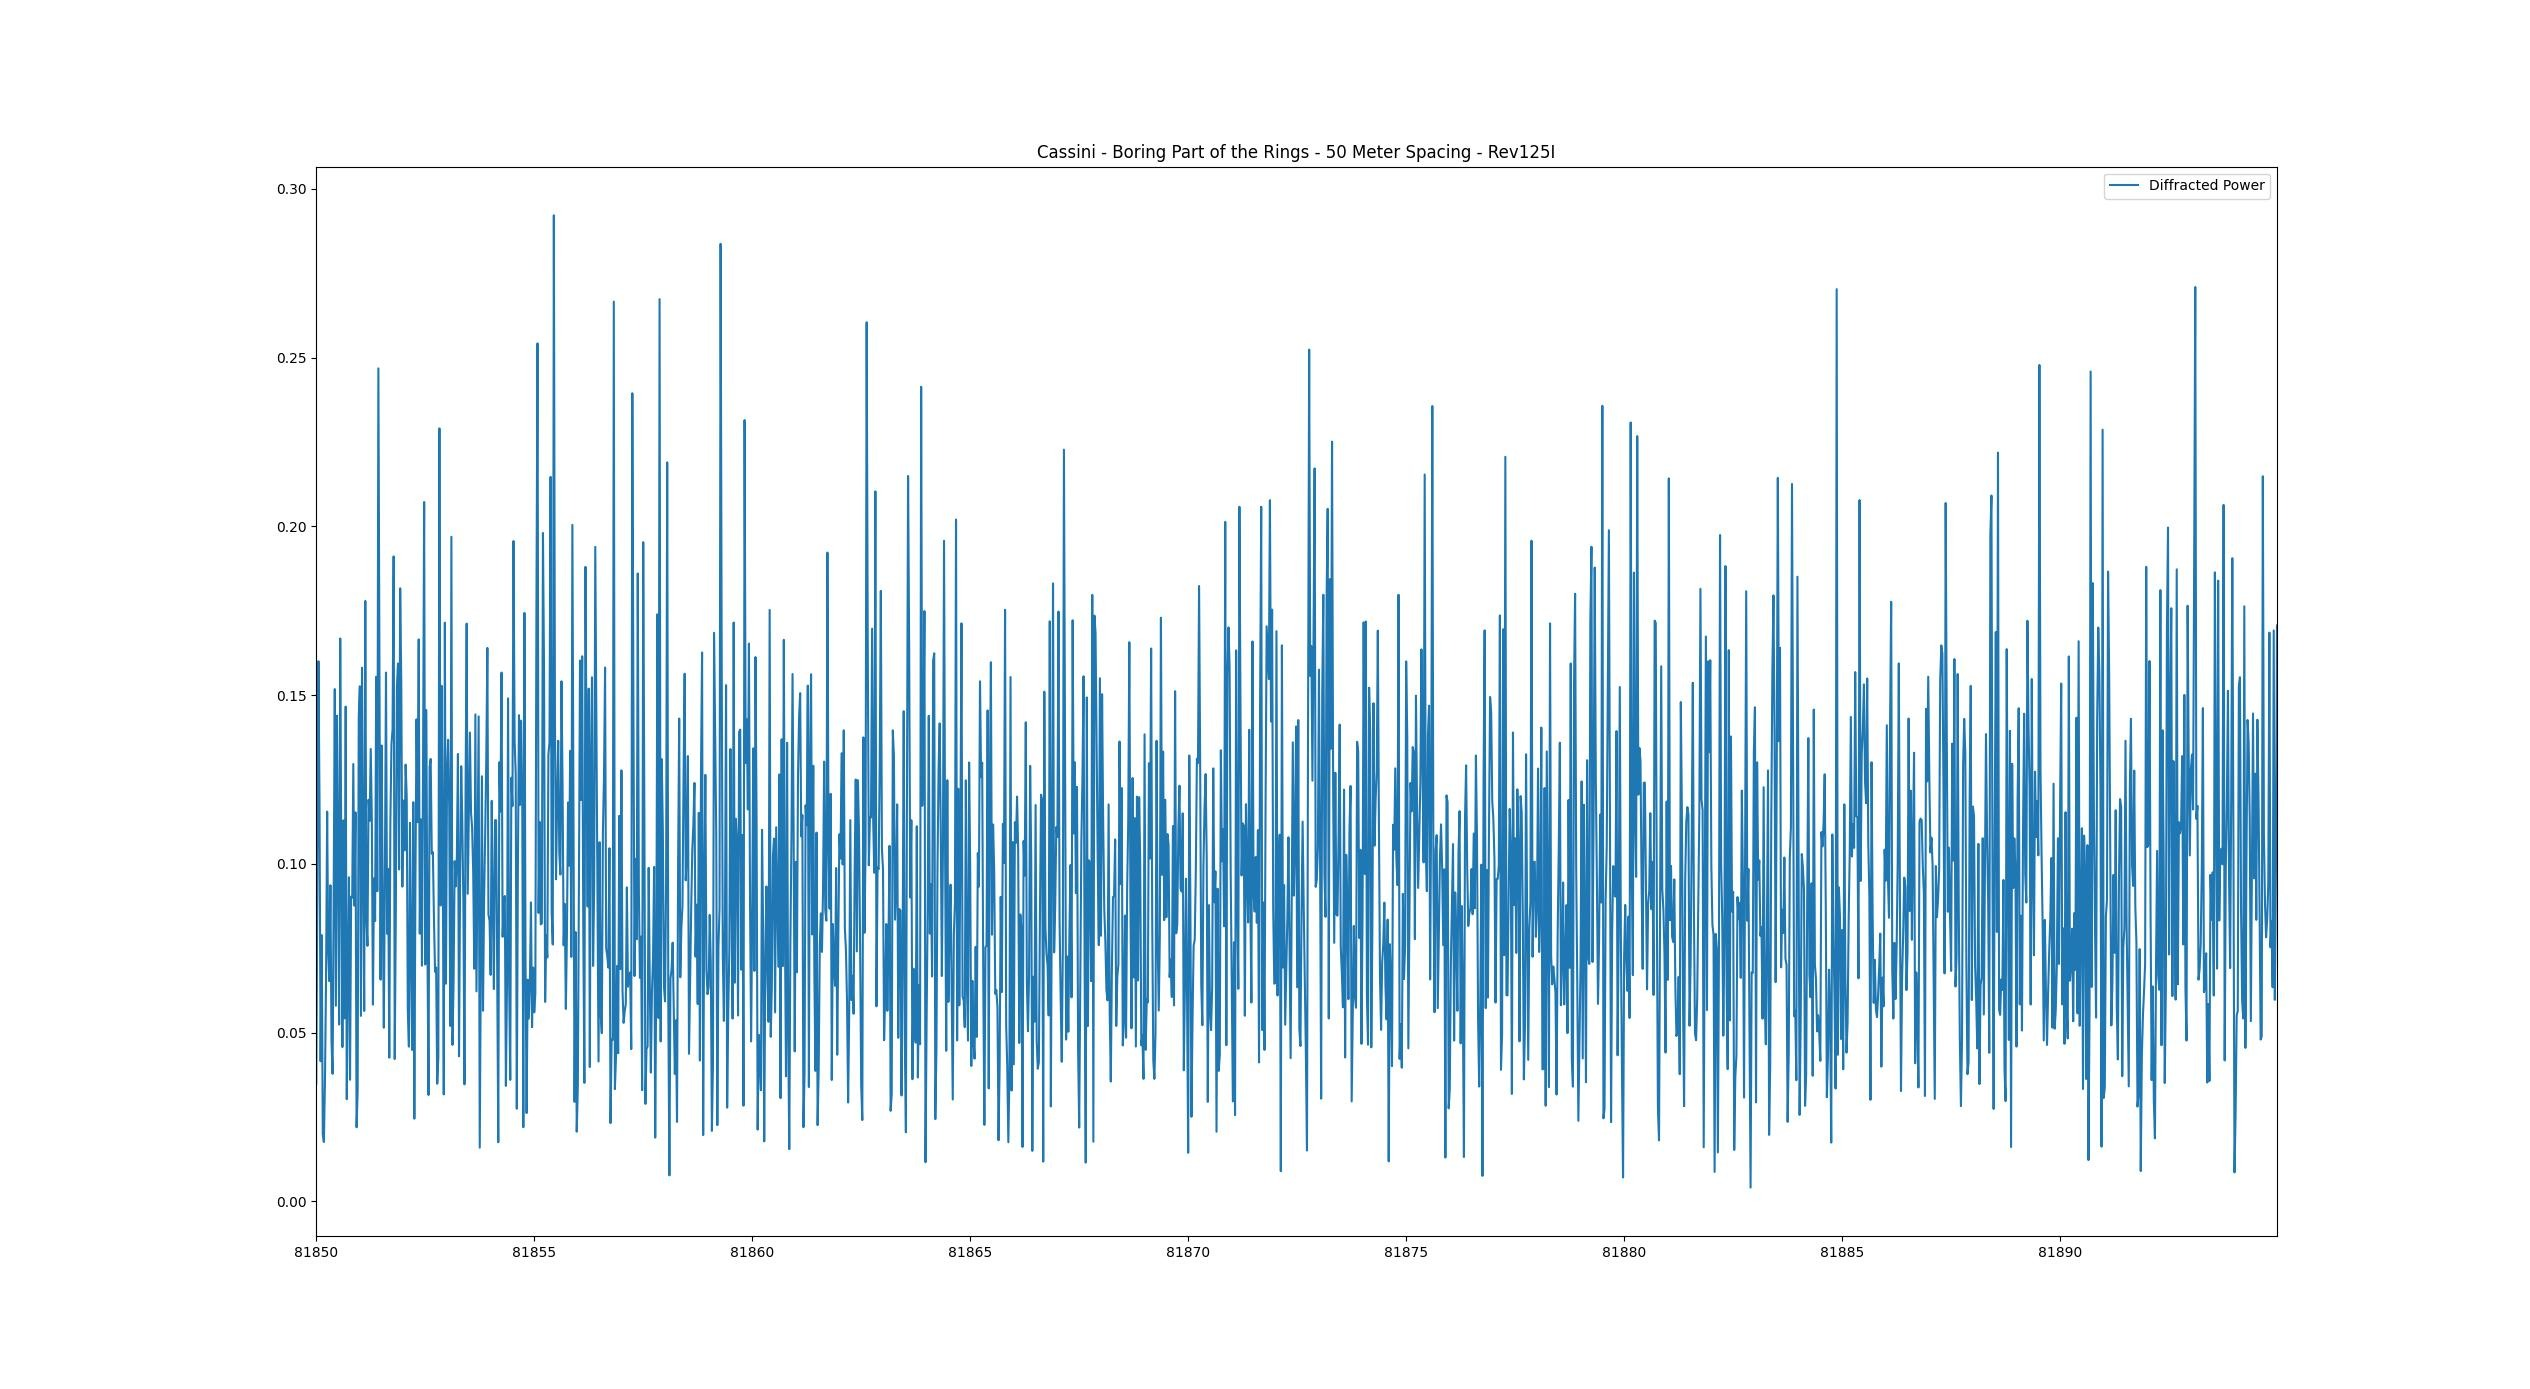
\includegraphics{cassini_boring_part_of_the_rings_diffracted_power.jpeg}}
        \end{figure}
    \end{frame}
    \begin{frame}{High Resolution with Low Opening Angle}
        This is what is on the NASA PDS
        (we swap to optical depth instead of power for this plot).
        \begin{figure}
            \resizebox{\textwidth}{!}{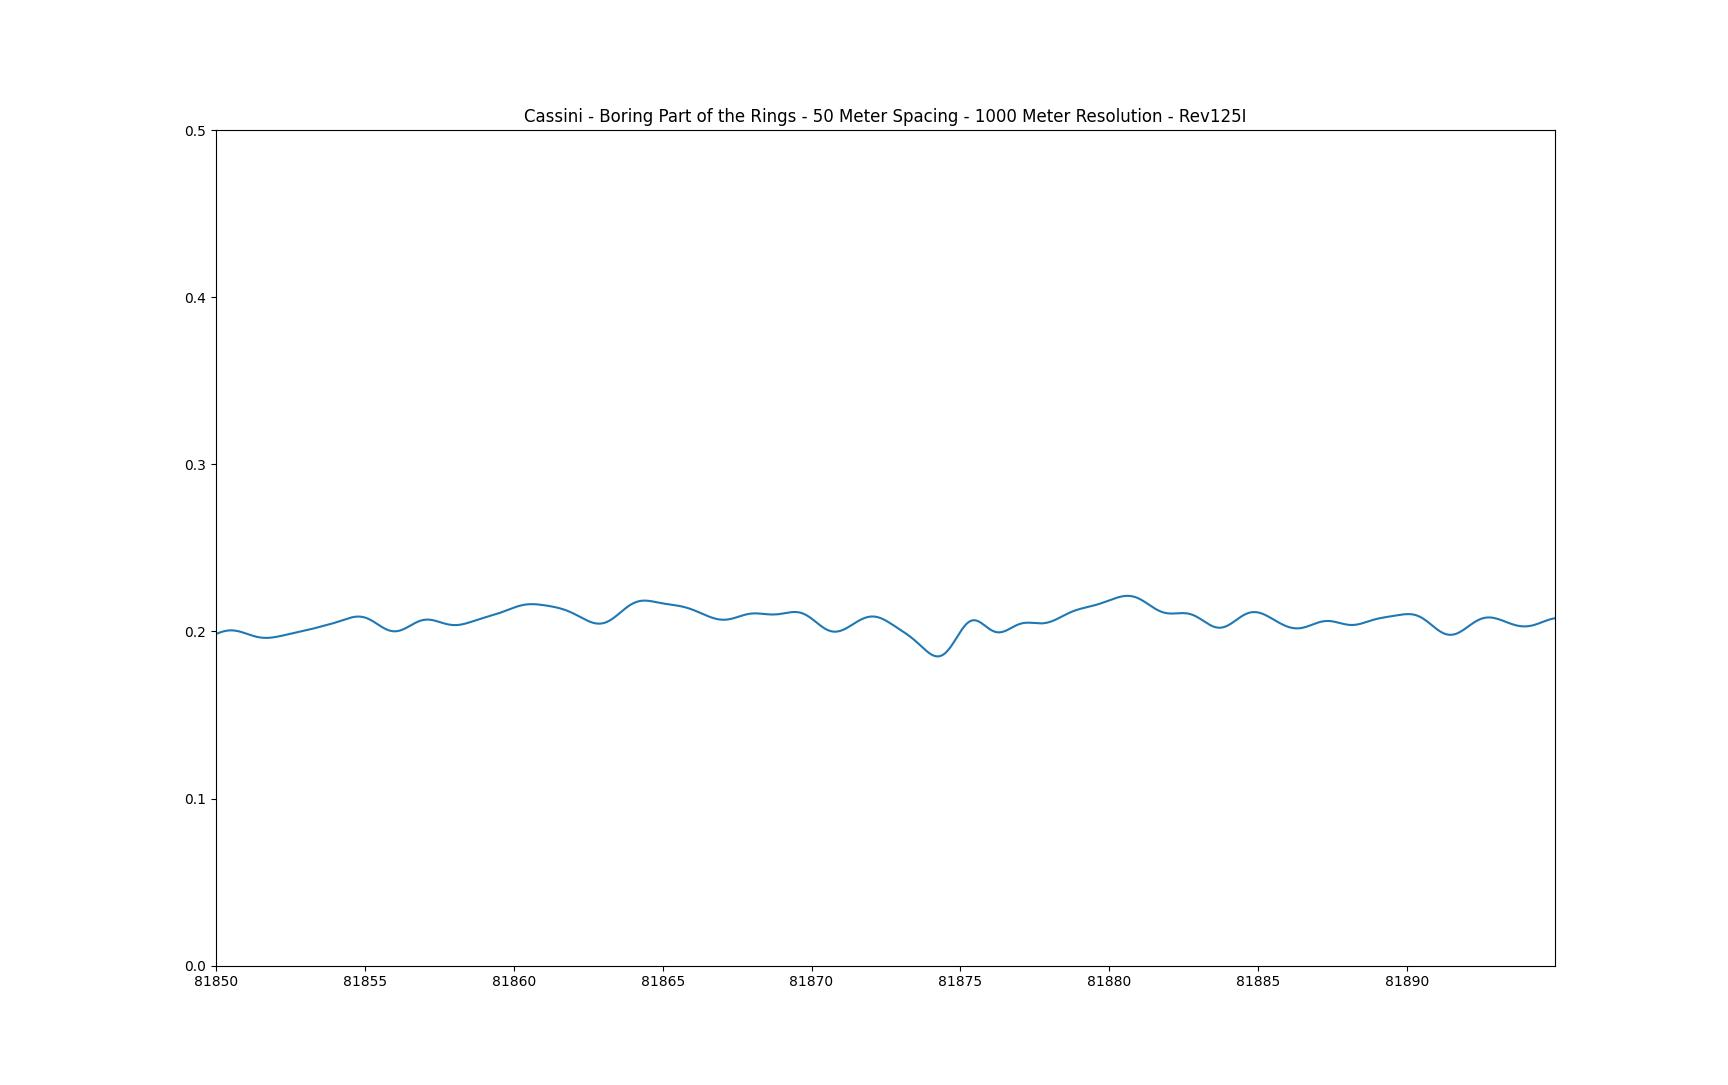
\includegraphics{cassini_boring_part_of_the_rings_optical_depth_1000m.png}}
        \end{figure}
    \end{frame}
    \begin{frame}{High Resolution with Low Opening Angle}
        Here's what we can do now!
        \begin{figure}
            \resizebox{\textwidth}{!}{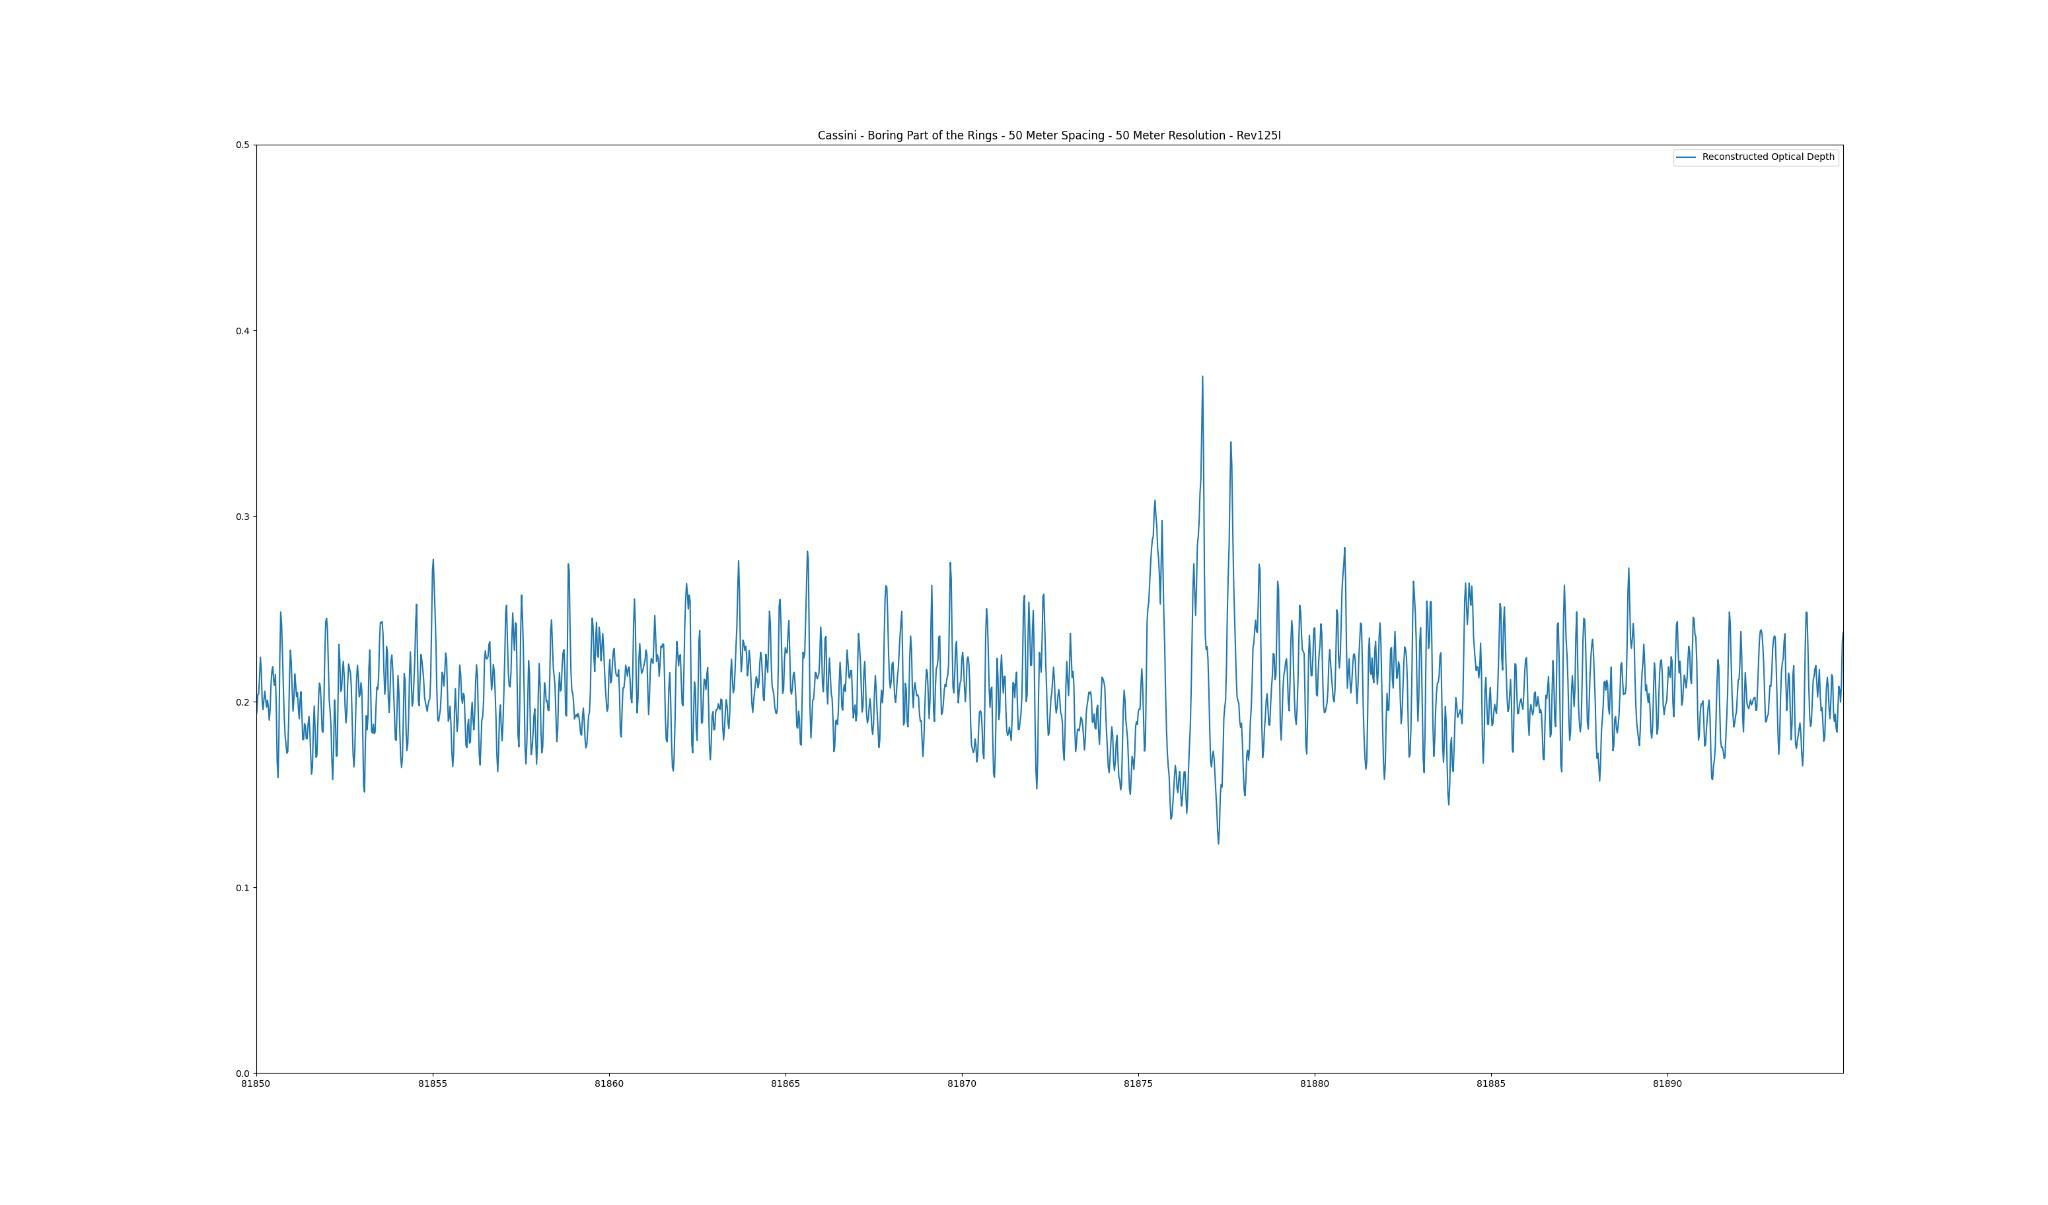
\includegraphics{cassini_boring_part_of_the_rings_optical_depth_50m.png}}
        \end{figure}
    \end{frame}
    \begin{frame}{High Resolution with Low Opening Angle}
        So, should you trust this?
    \end{frame}
    \begin{frame}{High Resolution with Low Opening Angle}
        I think so.
        \begin{figure}
            \resizebox{\textwidth}{!}{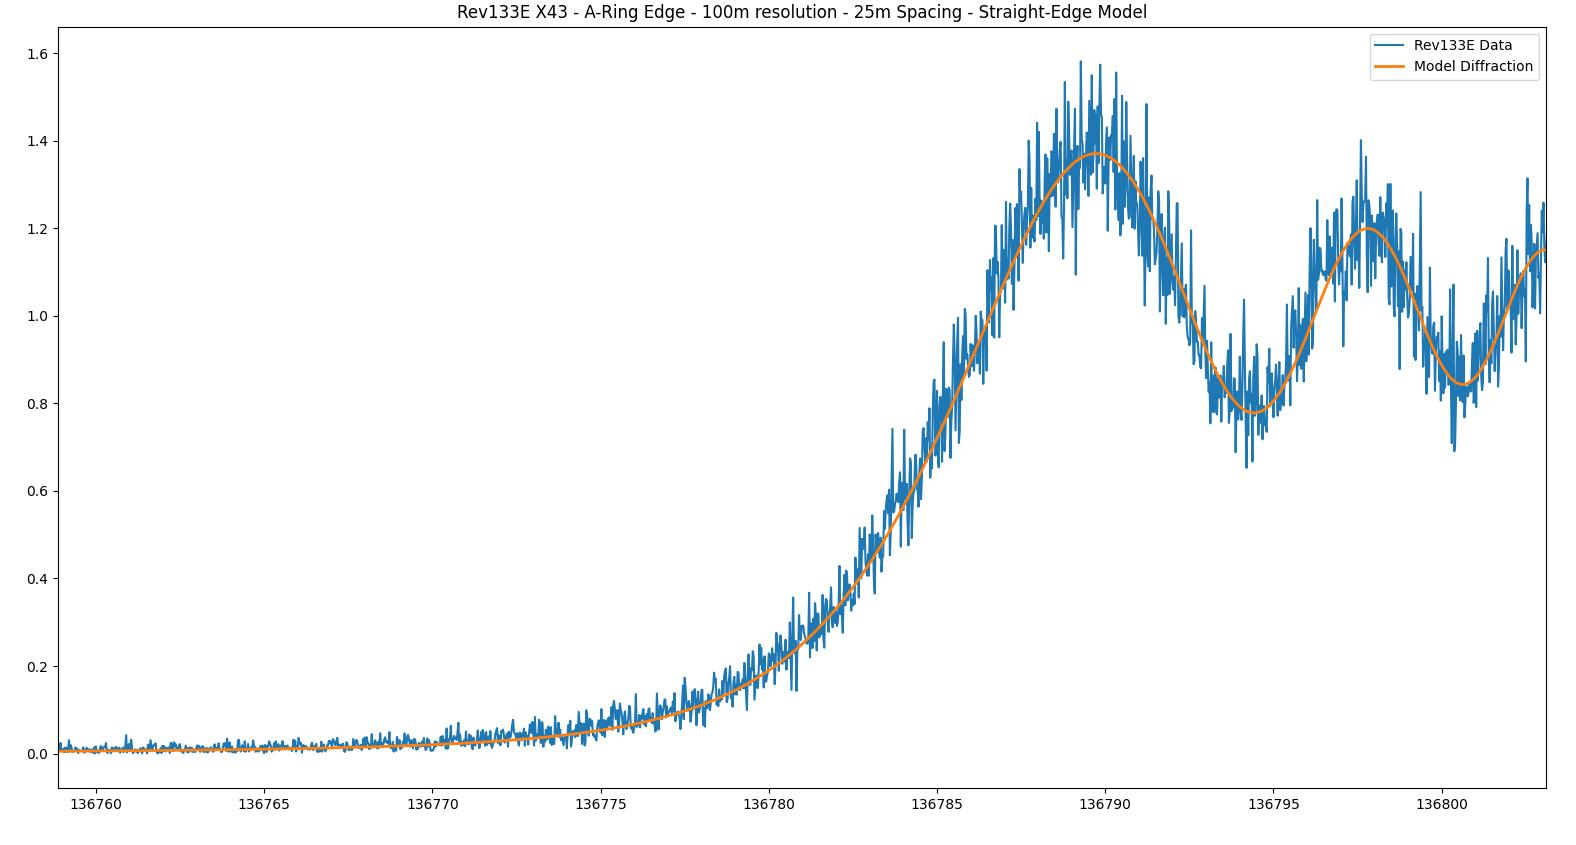
\includegraphics{cassini_rev133e_a_ring_model}}
        \end{figure}
    \end{frame}
    \begin{frame}{High Resolution with Low Opening Angle}
        The reconstruction.
        \begin{figure}
            \resizebox{\textwidth}{!}{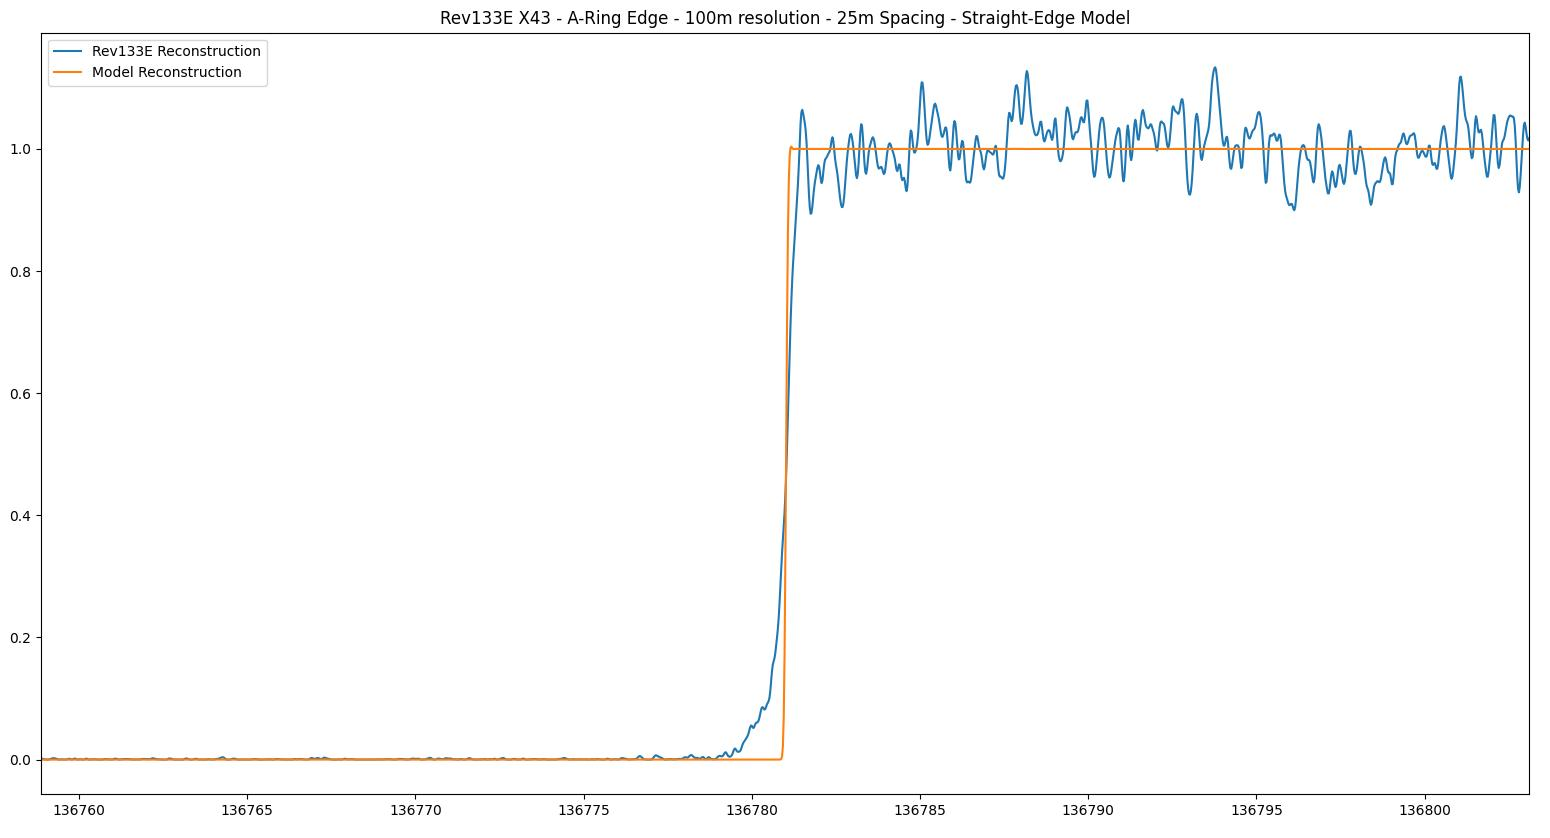
\includegraphics{cassini_rev133e_a_ring_reconstruction}}
        \end{figure}
    \end{frame}
    \begin{frame}{Some Problems Ahead...}
        We haven't resolved every issue. Are the rings truly symmetric?
        The moon Daphnis says \textit{no}.
        \begin{figure}
            \resizebox{0.8\textwidth}{!}{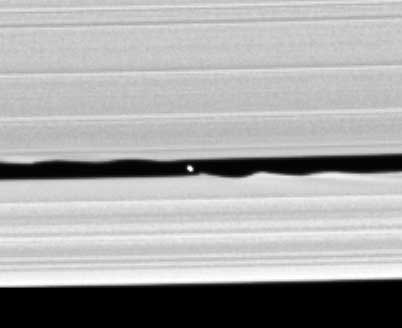
\includegraphics{moon_daphnis_from_cassini}}
        \end{figure}
    \end{frame}
    \begin{frame}{Some Problems Ahead...}
        Worse, the F ring is not even continuous! It's broken up in certain
        parts.
        \begin{figure}
            \resizebox{0.8\textwidth}{!}{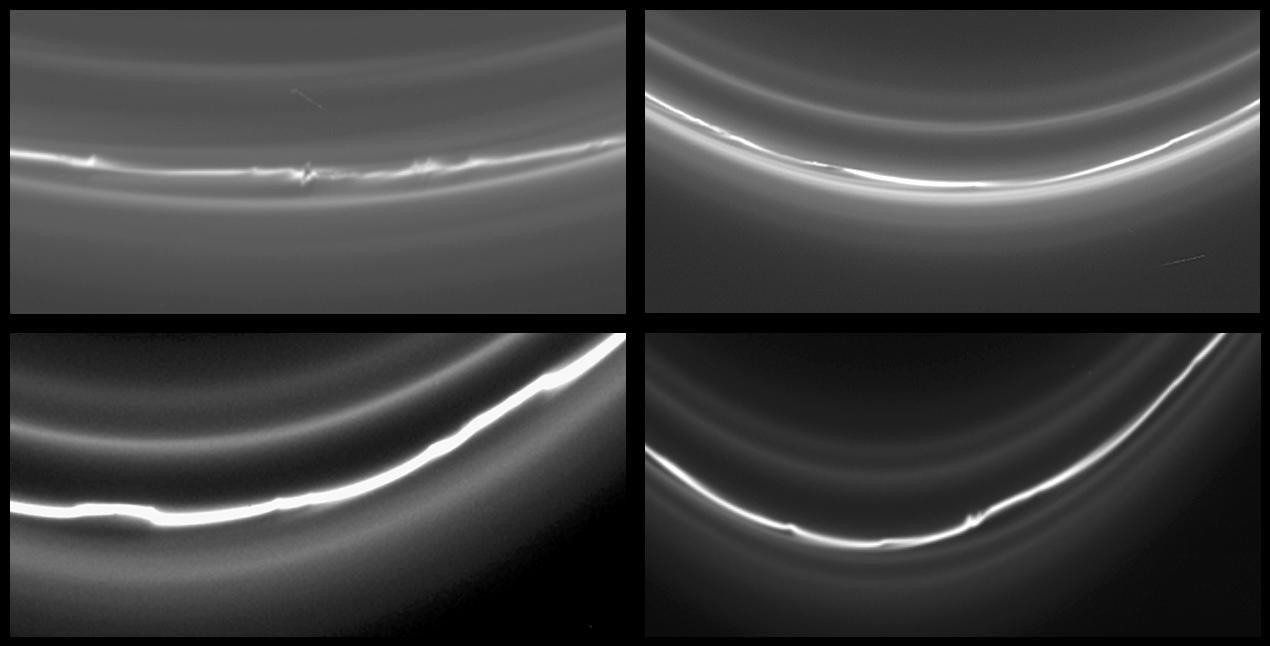
\includegraphics{saturn_f_ring}}
        \end{figure}
    \end{frame}
    \begin{frame}{Some Problems Ahead...}
        Hopefully in my next talk I'll have resolved these issues.
    \end{frame}
    \begin{frame}{The End}
        \begin{center}
            Thanks!
        \end{center}
    \end{frame}
\end{document}
